\chapter{The results of fits to \BdToKpill}
\label{all:swave:fits}


\section{Systematic contributions}



{\scriptsize
\begin{table}[tbp]
\caption{ \FL results + systematics ~\label{tbl:swave:meas:fl:results} }
\begin{tabular}{|c|c|c|c|c|c|c|c|c|}
\hline
 & 0.10 to  2.00: & 2.00 to  4.30: & 4.30 to  8.68: & 10.09 to  12.90: & 14.18 to  16.00: & 16.00 to  19.00: & 1.00 to  6.00: & 0.10 to  19.00:\\ 
val & 0.481 & 0.743 & 0.645 & 0.518 & 0.317 & 0.336 & 0.708 & 0.511\\ 
stat down & 0.074 & 0.074 & 0.056 & 0.059 & 0.063 & 0.066 & 0.057 & 0.027\\ 
stat up & 0.074 & 0.074 & 0.056 & 0.059 & 0.063 & 0.066 & 0.057 & 0.027\\ 
sys down & 0.0507 & 0.0326 & 0.0514 & 0.073 & 0.0345 & 0.0366 & 0.0472 & 0.0511\\ 
sys up & 0.0323 & 0.0538 & 0.0337 & 0.0287 & 0.0253 & 0.0273 & 0.0351 & 0.0304\\ 
doublegaus & -0.025 & -0.018 & -0.03 & -0.036 & -0.012 & -0.008 & -0.027 & -0.026\\ 
triggerup & 0 & 0 & 0 & 0 & 0 & 0 & 0 & 0\\ 
triggerdown & 0 & 0 & 0 & 0 & 0 & 0 & 0 & 0\\ 
trackingup & 0.002 & 0.001 & 0.003 & 0.002 & 0.001 & 0.001 & 0.001 & 0.001\\ 
trackingdown & -0.001 & -0.002 & -0.002 & -0.002 & -0.001 & -0.001 & -0.002 & -0.001\\ 
muonup & 0 & 0 & 0 & 0 & 0 & 0 & 0 & 0\\ 
dllsysdown & -0.006 & -0.002 & -0.009 & -0.018 & -0.01 & -0.014 & -0.005 & -0.009\\ 
bkgpoly & -0.025 & -0.017 & -0.028 & -0.035 & -0.011 & -0.008 & -0.027 & -0.025\\ 
noips & 0.004 & 0.007 & 0.013 & 0.006 & 0.004 & 0.011 & 0.012 & 0.009\\ 
muondown & 0 & 0 & 0 & 0 & 0 & 0 & 0 & 0\\ 
lass & -0.021 & 0.049 & -0.002 & -0.039 & -0.016 & -0.017 & 0.019 & -0.022\\ 
syctkup & -0.029 & -0.021 & -0.028 & -0.026 & -0.022 & -0.023 & -0.027 & -0.026\\ 
sysctkdown & 0.032 & 0.021 & 0.031 & 0.028 & 0.025 & 0.025 & 0.027 & 0.029\\ 
dllsysup & -0.002 & -0.002 & -0.009 & -0.017 & -0.009 & -0.014 & -0.004 & -0.008\\ 
\hline
\end{tabular}
\end{table}


\begin{table}[tbp]
\caption{ \FS results + systematics ~\label{tbl:swave:meas:fs:results} }
\begin{tabular}{|c|c|c|c|c|c|c|c|c|}
\hline
 & 0.10 to  2.00: & 2.00 to  4.30: & 4.30 to  8.68: & 10.09 to  12.90: & 14.18 to  16.00: & 16.00 to  19.00: & 1.00 to  6.00: & 0.10 to  19.00:\\ 
val & 0.195 & 0.236 & 0.237 & 0.142 & 0.064 & 0.06 & 0.124 & 0.161\\ 
stat down & 0.039 & 0.056 & 0.03 & 0.03 & 0.023 & 0.02 & 0.018 & 0.014\\ 
stat up & -0.037 & -0.057 & -0.03 & -0.03 & -0.023 & -0.02 & -0.017 & -0.013\\ 
sys down & 0.001 & 0.0118 & 0.006 & 0.0444 & 0.048 & 0.0571 & 0.00728 & 0.0186\\ 
sys up & 0.126 & 0.184 & 0.0724 & 0.00412 & 0.00224 & 0.001 & 0.0882 & 0.00458\\ 
doublegaus & 0.004 & -0.01 & -0.001 & -0.009 & -0.001 & -0.001 & -0.005 & -0.002\\ 
triggerup & 0 & 0 & 0 & 0 & 0 & 0 & 0 & 0\\ 
triggerdown & 0 & 0 & 0 & 0 & 0 & 0 & 0 & 0\\ 
trackingup & 0 & 0.001 & -0.001 & 0.001 & 0 & 0 & 0 & 0\\ 
trackingdown & 0.001 & -0.001 & 0 & 0 & 0 & 0 & -0.001 & 0\\ 
muonup & 0 & 0 & 0 & 0 & 0 & 0 & 0 & 0\\ 
dllsysdown & 0 & -0.001 & -0.003 & -0.004 & 0 & -0.001 & -0.001 & -0.002\\ 
bkgpoly & 0.005 & -0.001 & 0.003 & 0 & 0.002 & -0.002 & -0.003 & 0.001\\ 
noips & 0.001 & 0.006 & 0.005 & 0 & 0 & -0.001 & 0.004 & 0.002\\ 
muondown & 0 & 0 & 0 & 0 & 0 & 0 & 0 & 0\\ 
lass & 0.126 & 0.184 & 0.072 & -0.043 & -0.048 & -0.057 & 0.088 & -0.018\\ 
sysctkup & 0.001 & -0.006 & -0.004 & -0.003 & -0.001 & -0.001 & 0.004 & -0.003\\ 
sysctkdown & -0.001 & 0.006 & 0.005 & 0.004 & 0.001 & 0.001 & -0.004 & 0.004\\ 
dllsysup & 0 & 0 & -0.003 & -0.004 & 0 & 0 & -0.001 & -0.002\\ 
\hline
\end{tabular}
\end{table}




\begin{table}[tbp]
\caption{ \ASi results + systematics ~\label{tbl:swave:meas:as:results} }
\begin{tabular}{|c|c|c|c|c|c|c|c|c|}
\hline
 & 0.10 to  2.00: & 2.00 to  4.30: & 4.30 to  8.68: & 10.09 to  12.90: & 14.18 to  16.00: & 16.00 to  19.00: & 1.00 to  6.00: & 0.10 to  19.00:\\ 
val & 0.31 & -0.19 & -0.093 & 0.222 & 0.363 & 0.559 & 0.172 & 0.084\\ 
stat down & 0.18 & 0.268 & 0.136 & 0.205 & 0.287 & 0.3 & 0.14 & 0.08\\ 
stat up & 0.18 & 0.268 & 0.136 & 0.205 & 0.287 & 0.3 & 0.14 & 0.08\\ 
sys down & 0.157 & 0.0415 & 0.0272 & 0.0186 & 0.0275 & 0.0736 & 0.0398 & 0.0279\\ 
sys up & 0.151 & 0.527 & 0.161 & 0.446 & 0.145 & 0.301 & 0.192 & 0.203\\ 
doublegaus & 0.106 & 0.137 & 0.114 & 0.142 & 0.062 & 0.036 & 0.111 & 0.113\\ 
triggerup & 0 & 0 & 0 & 0 & 0 & 0 & 0 & 0\\ 
triggerdown & 0 & 0 & 0 & 0 & 0 & 0 & 0 & 0\\ 
trackingup & -0.008 & -0.011 & -0.009 & -0.008 & -0.001 & 0.001 & -0.008 & -0.007\\ 
trackingdown & 0.012 & 0.01 & 0.008 & 0.007 & 0.001 & -0.001 & 0.008 & 0.006\\ 
muonup & 0 & 0 & 0 & 0 & 0 & 0 & 0 & 0\\ 
dllsysdown & 0.006 & 0.013 & 0.02 & 0.044 & 0.005 & -0.058 & 0.009 & 0.012\\ 
bkgpoly & 0.107 & 0.139 & 0.109 & 0.109 & 0.051 & 0.04 & 0.109 & 0.107\\ 
noips & -0.031 & -0.04 & -0.025 & -0.016 & -0.023 & 0.009 & -0.039 & -0.027\\ 
muondown & 0 & 0 & 0 & 0 & 0 & 0 & 0 & 0\\ 
lass & -0.154 & 0.489 & 0.008 & 0.404 & 0.12 & 0.295 & 0.111 & 0.129\\ 
sysctkup & -0.001 & -0.001 & 0.004 & -0.005 & -0.015 & -0.017 & 0 & 0\\ 
sysctkdown & 0.001 & 0.001 & -0.006 & 0.002 & 0.016 & 0.022 & 0 & 0\\ 
dllsysup & 0.006 & 0.009 & 0.022 & 0.045 & 0.002 & -0.042 & 0.008 & 0.015\\ 
\hline
\end{tabular}
\end{table}
}
\clearpage

\section{LASS model}

\begin{figure}[tbp]
\centering
\subfigure{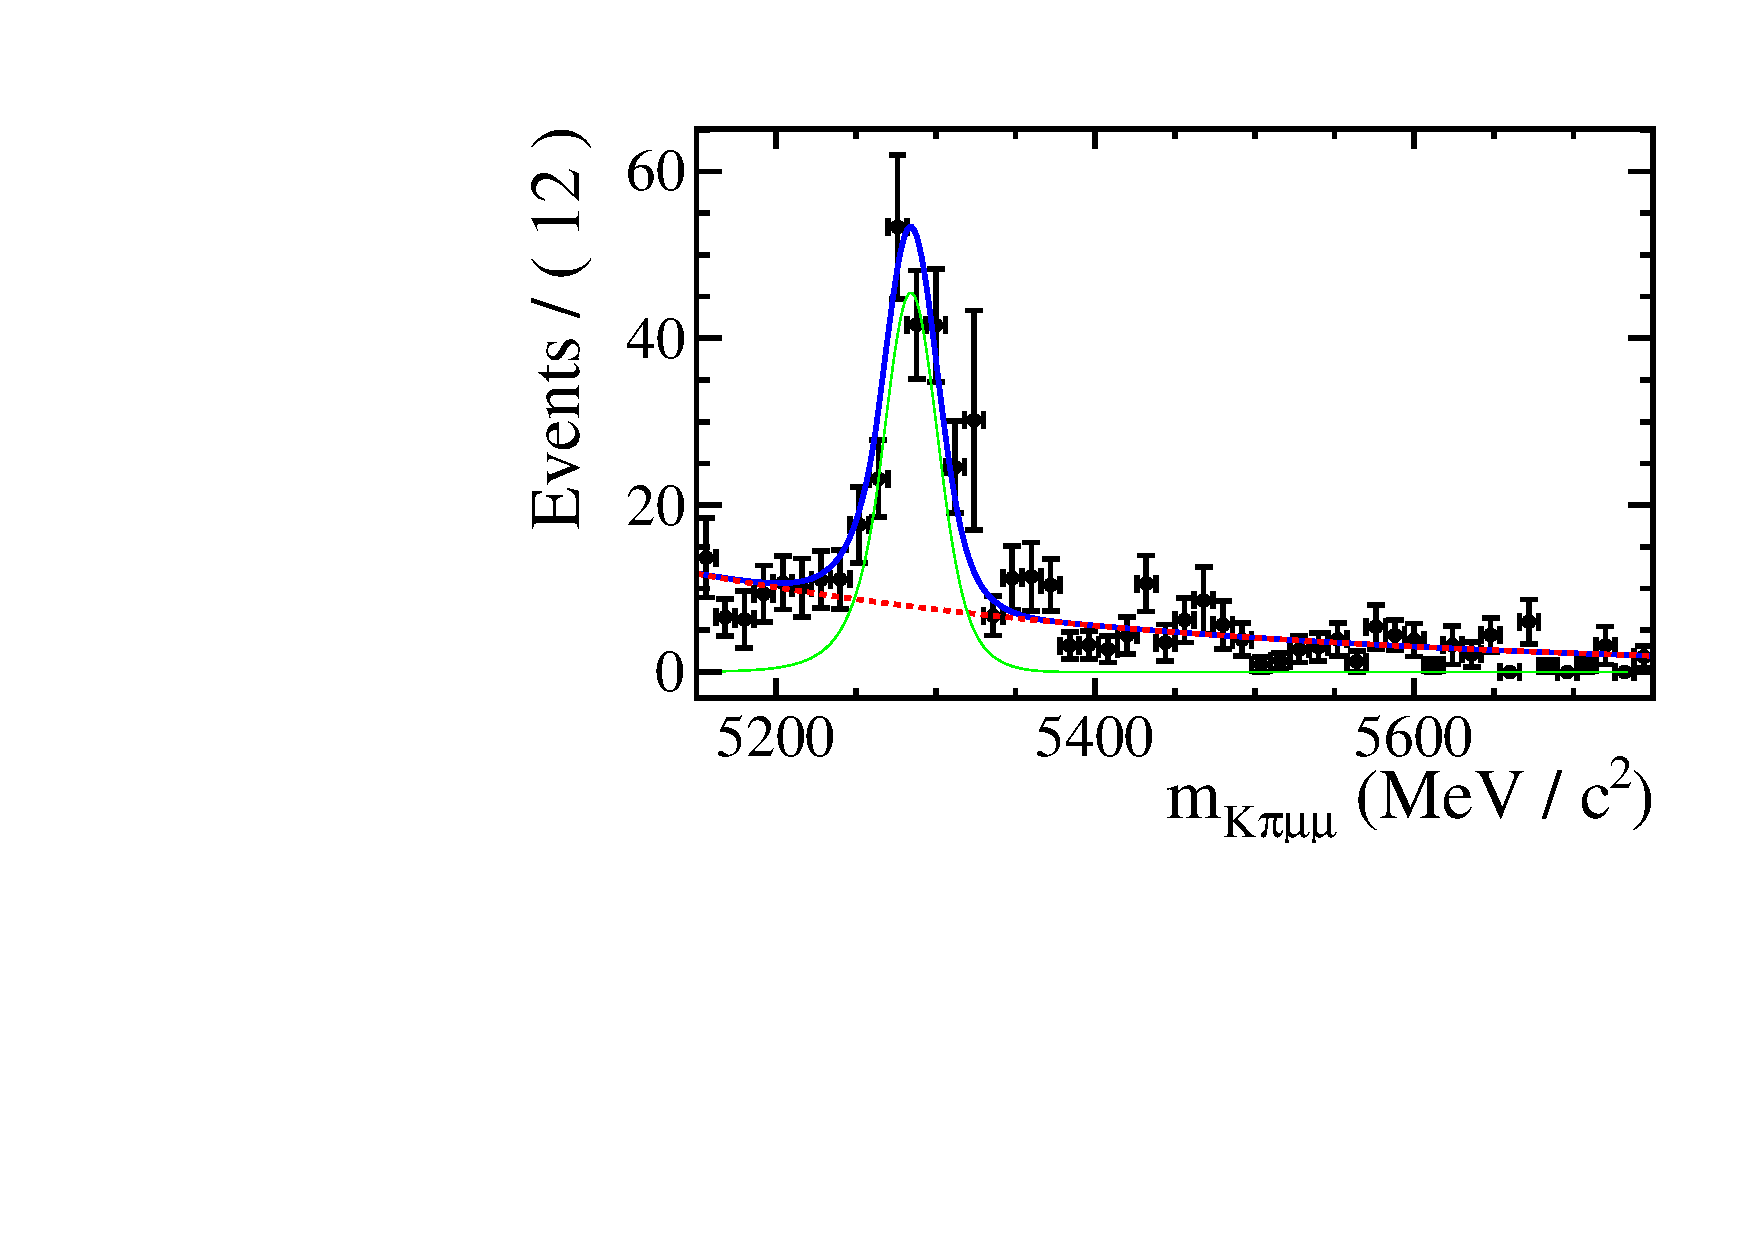
\includegraphics[width=0.48\columnwidth]
{chapter7/figs/fits/lass/fit_kstarmumu_swave_mkpi_range_lass_mass_canvas_0.pdf}}
\subfigure{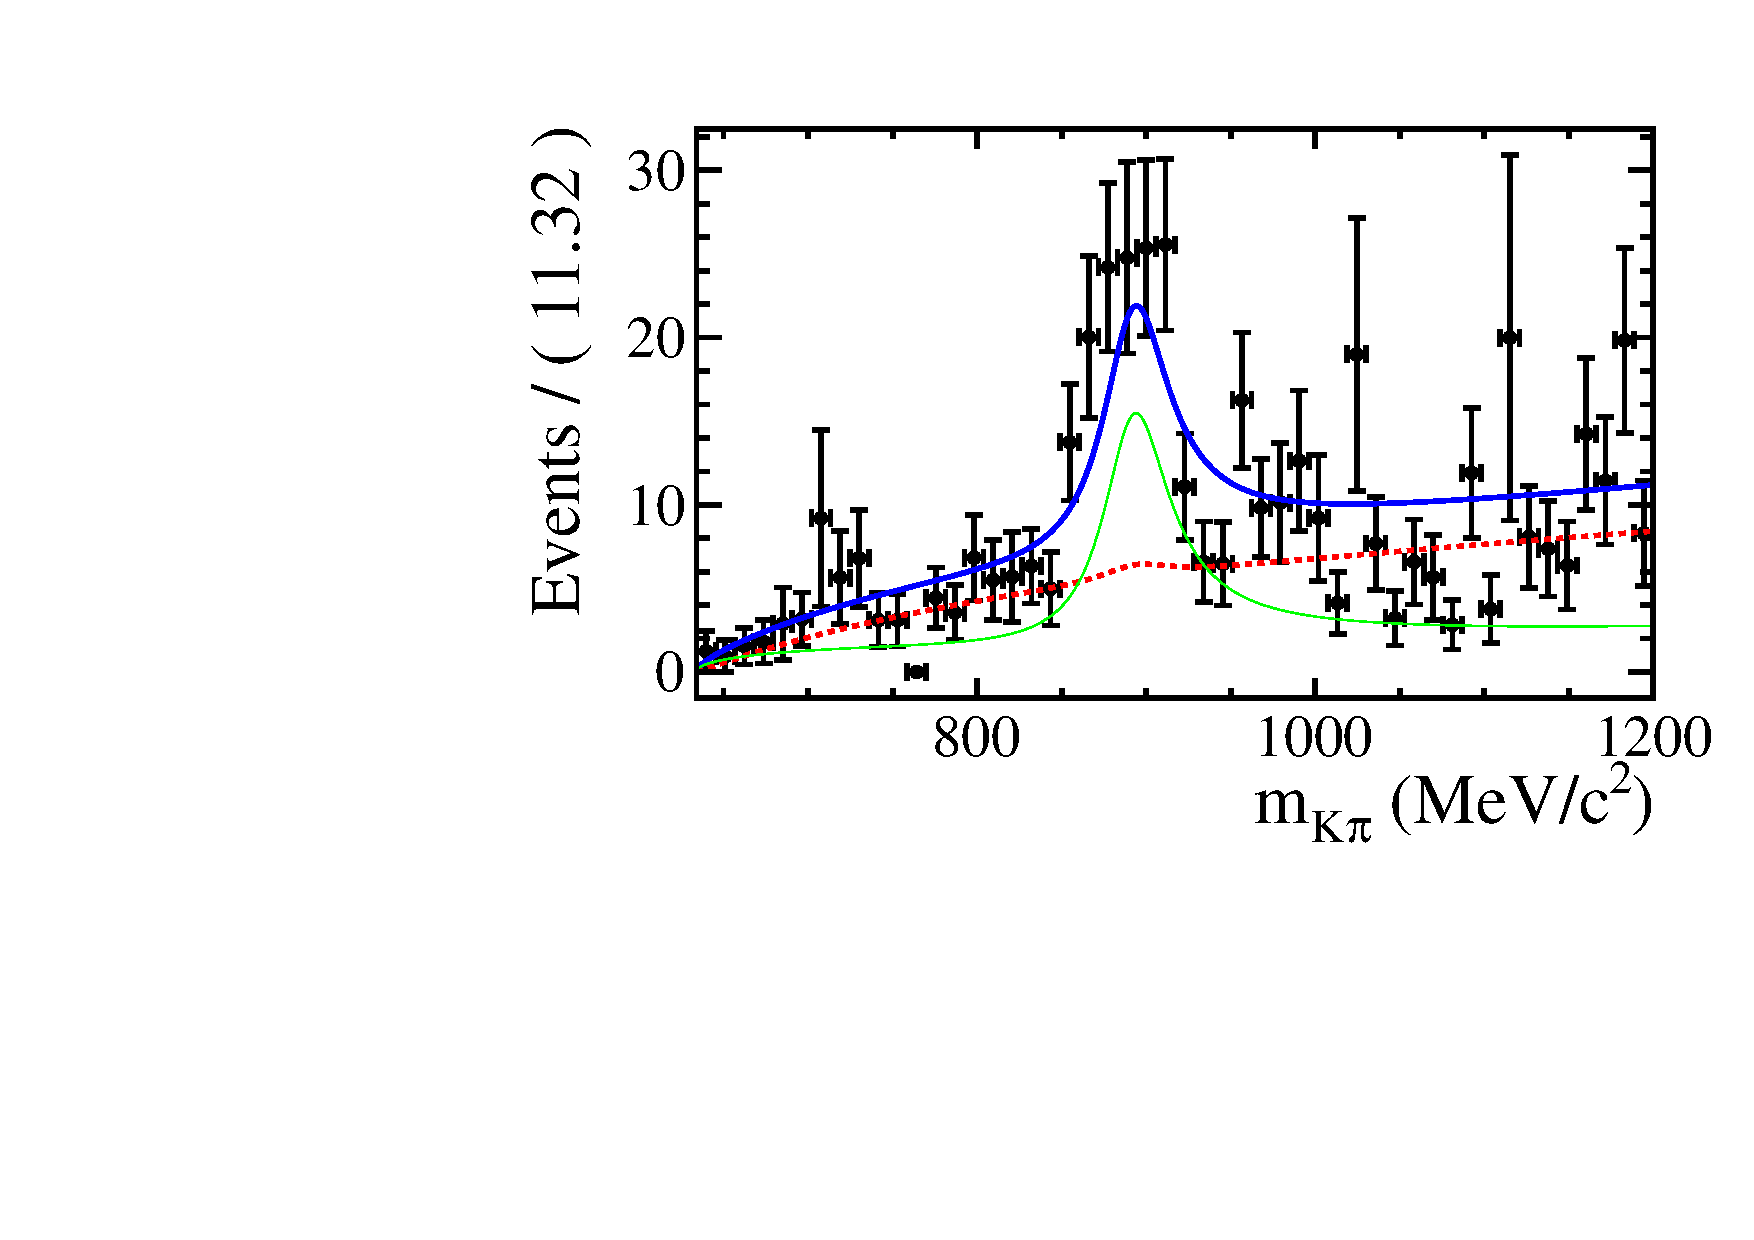
\includegraphics[width=0.48\columnwidth]
{chapter7/figs/fits/lass/fit_kstarmumu_swave_mkpi_range_lass_mkpi_canvas_0.pdf}}
\subfigure{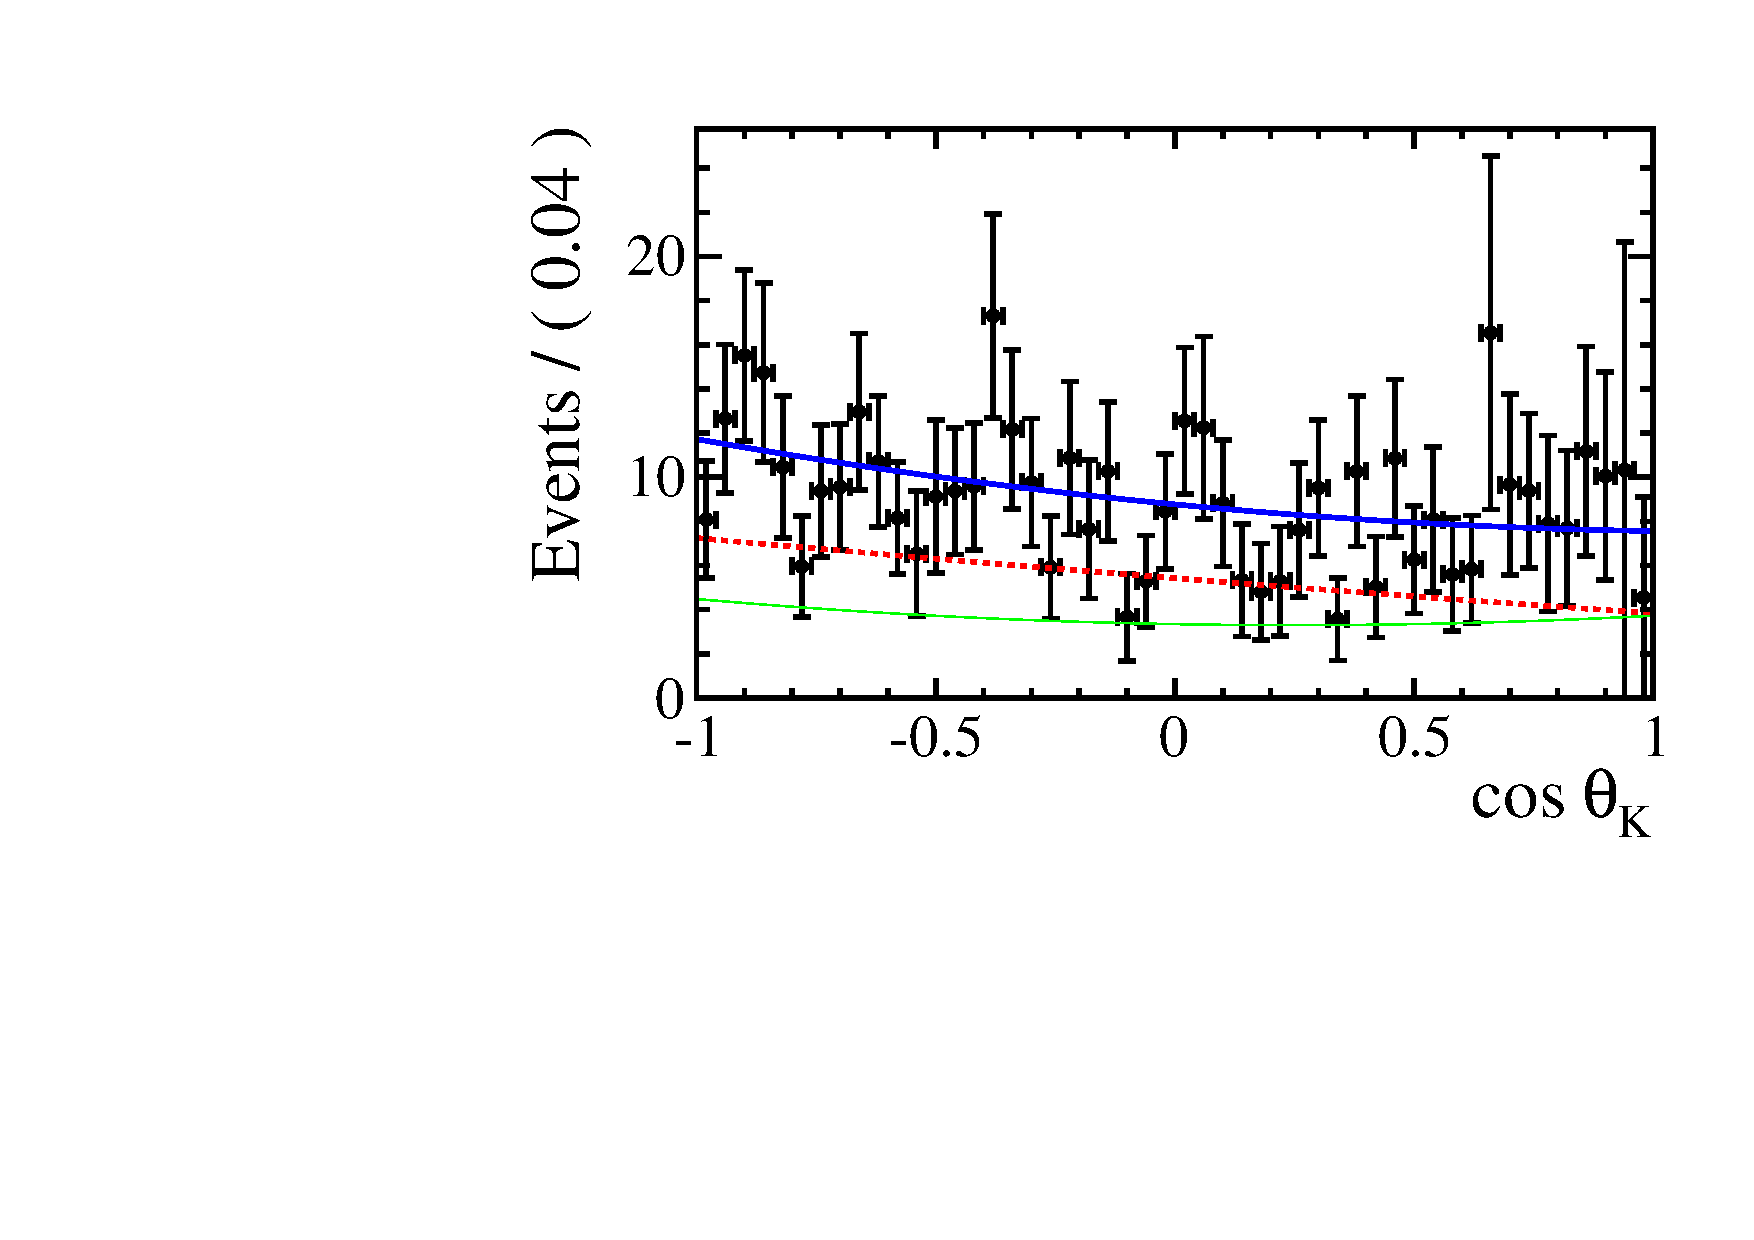
\includegraphics[width=0.48\columnwidth]
{chapter7/figs/fits/lass/fit_kstarmumu_swave_mkpi_range_lass_costhetak_canvas_0.pdf}}
\caption{ The result of the fit to the \qsq region from 0.1 to 2 \gevgevcccc. }
\end{figure}

\begin{figure}[tbp]
\centering
\subfigure{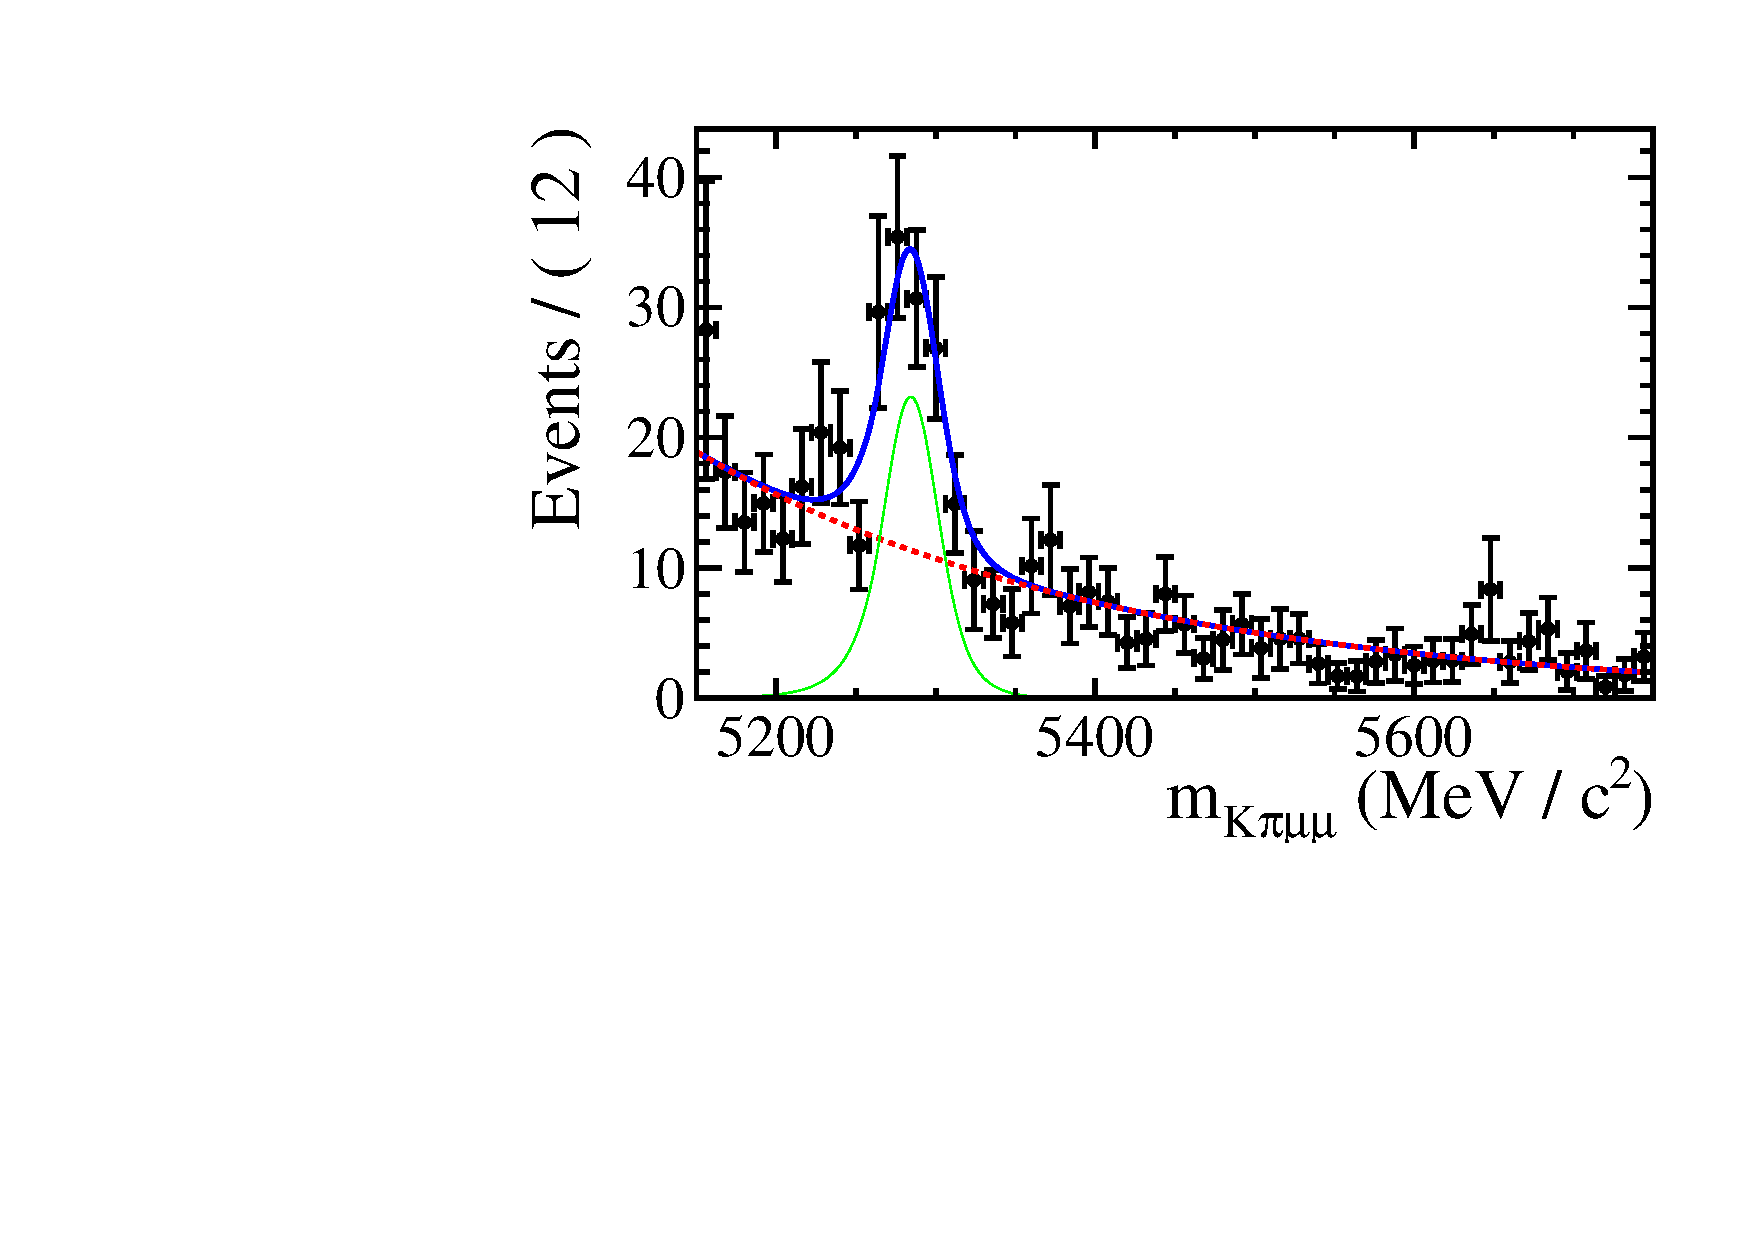
\includegraphics[width=0.48\columnwidth]
{chapter7/figs/fits/lass/fit_kstarmumu_swave_mkpi_range_lass_mass_canvas_1.pdf}}
\subfigure{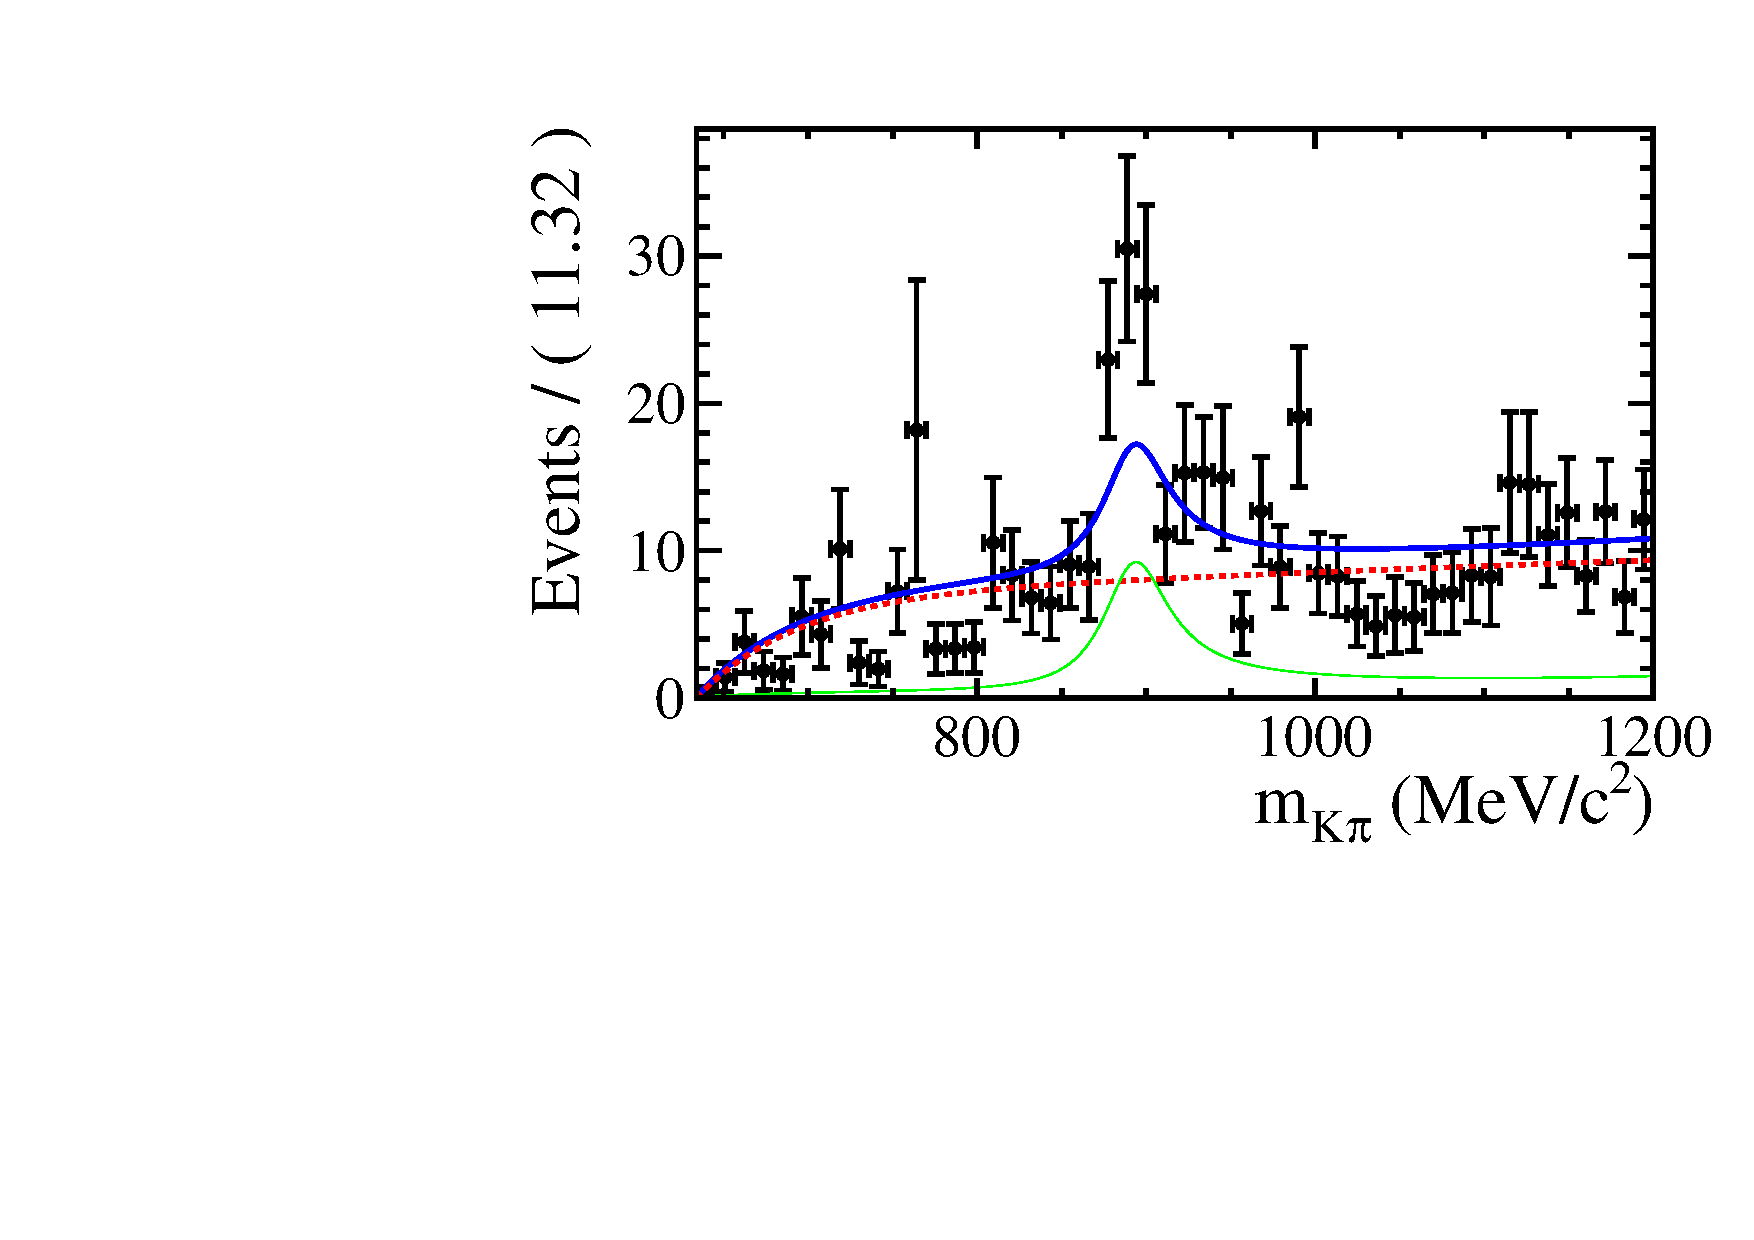
\includegraphics[width=0.48\columnwidth]
{chapter7/figs/fits/lass/fit_kstarmumu_swave_mkpi_range_lass_mkpi_canvas_1.pdf}}
\subfigure{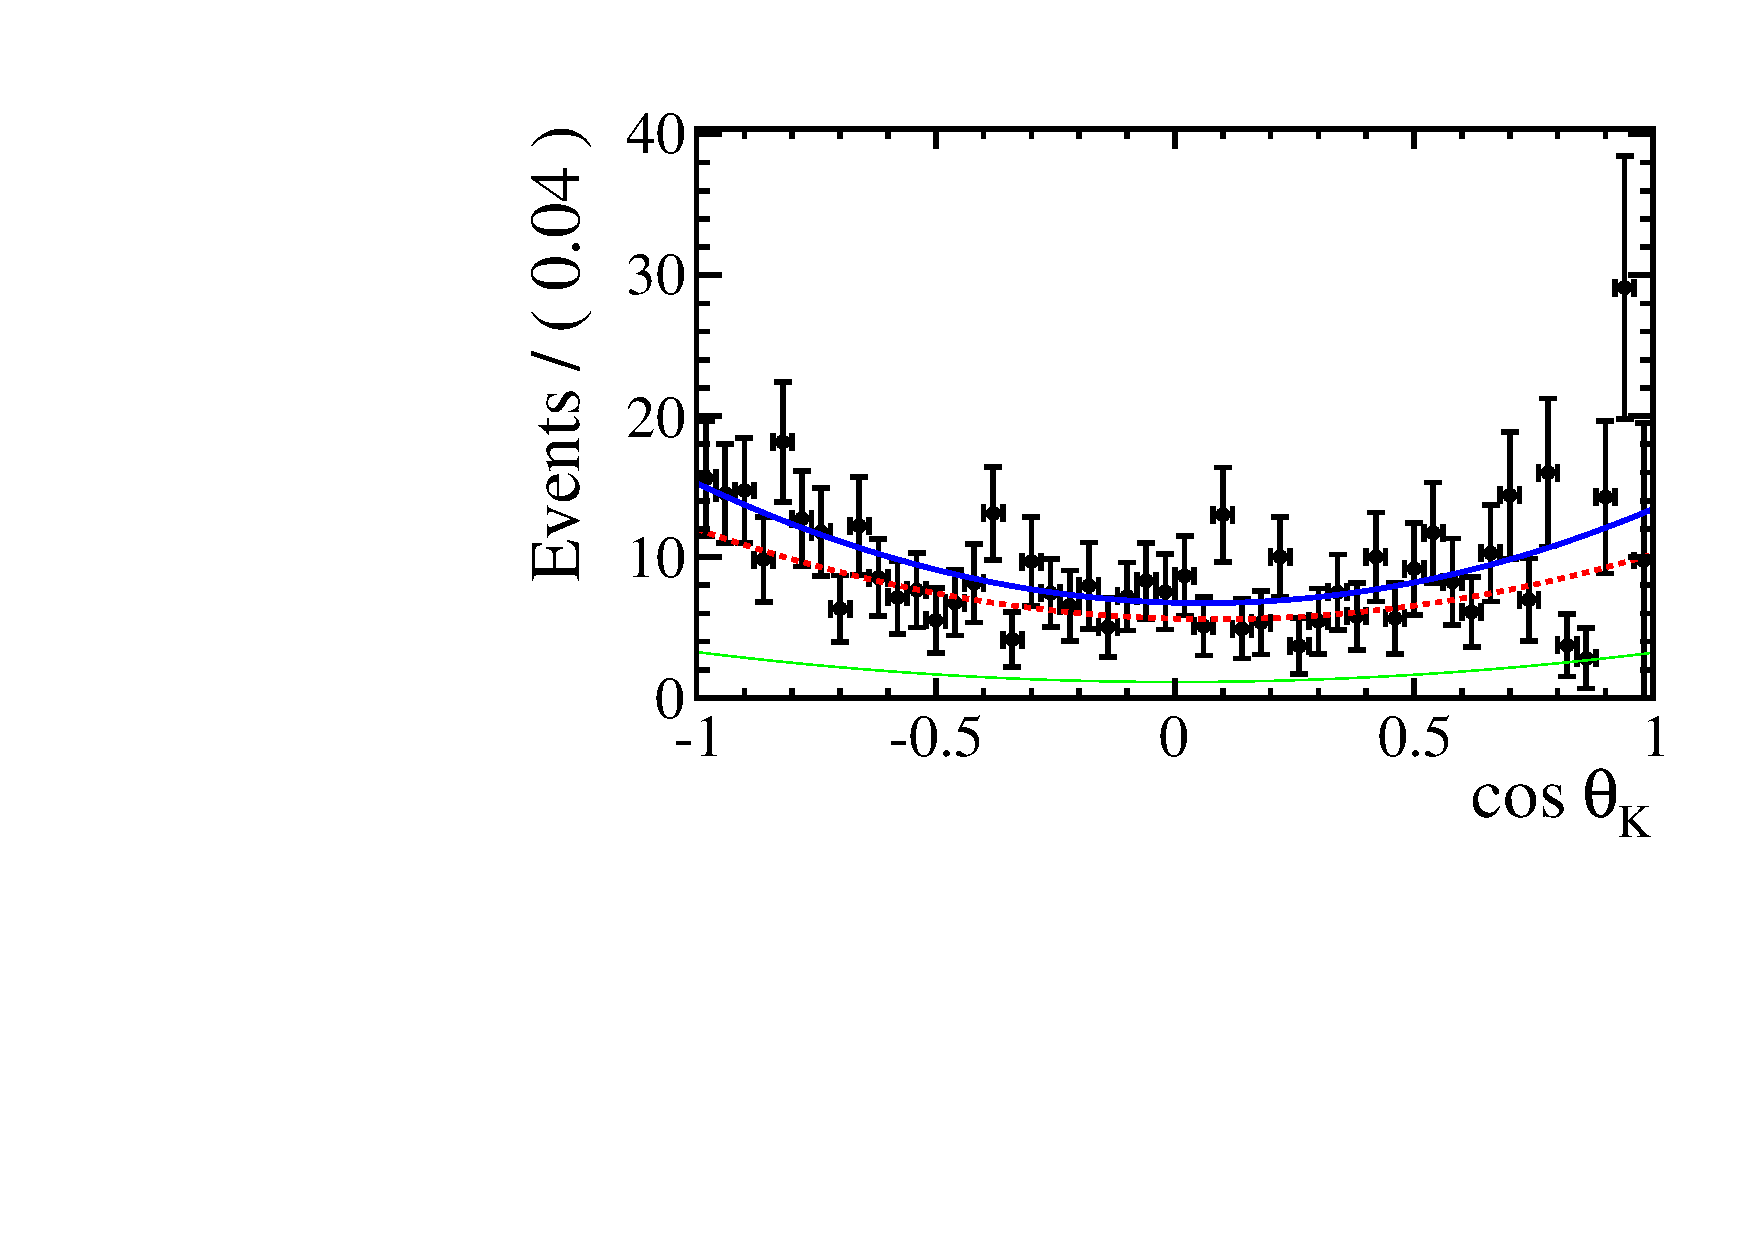
\includegraphics[width=0.48\columnwidth]
{chapter7/figs/fits/lass/fit_kstarmumu_swave_mkpi_range_lass_costhetak_canvas_1.pdf}}
\caption{ The result of the fit to the \qsq region from 2 to 4.3 \gevgevcccc. }
\end{figure}

\begin{figure}[tbp]
\centering
\subfigure{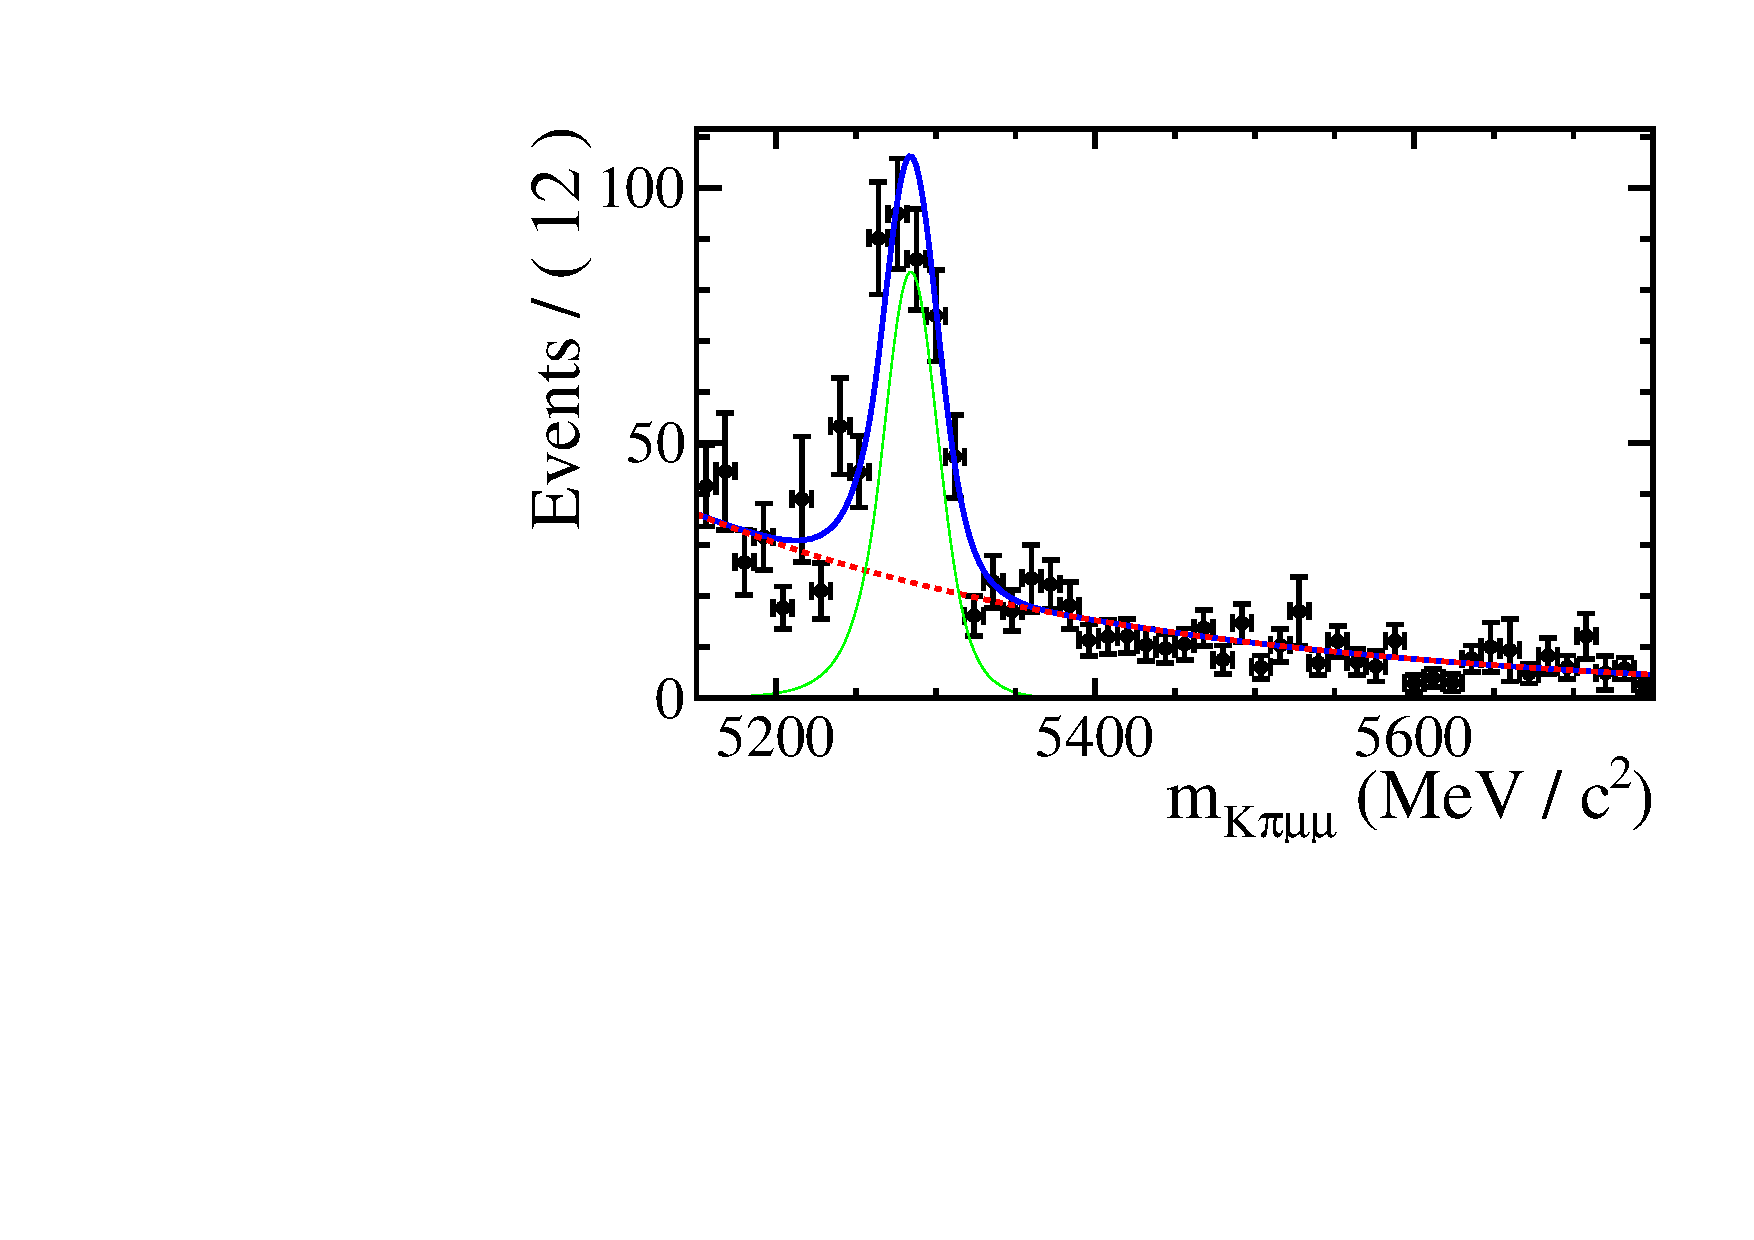
\includegraphics[width=0.48\columnwidth]
{chapter7/figs/fits/lass/fit_kstarmumu_swave_mkpi_range_lass_mass_canvas_2.pdf}}
\subfigure{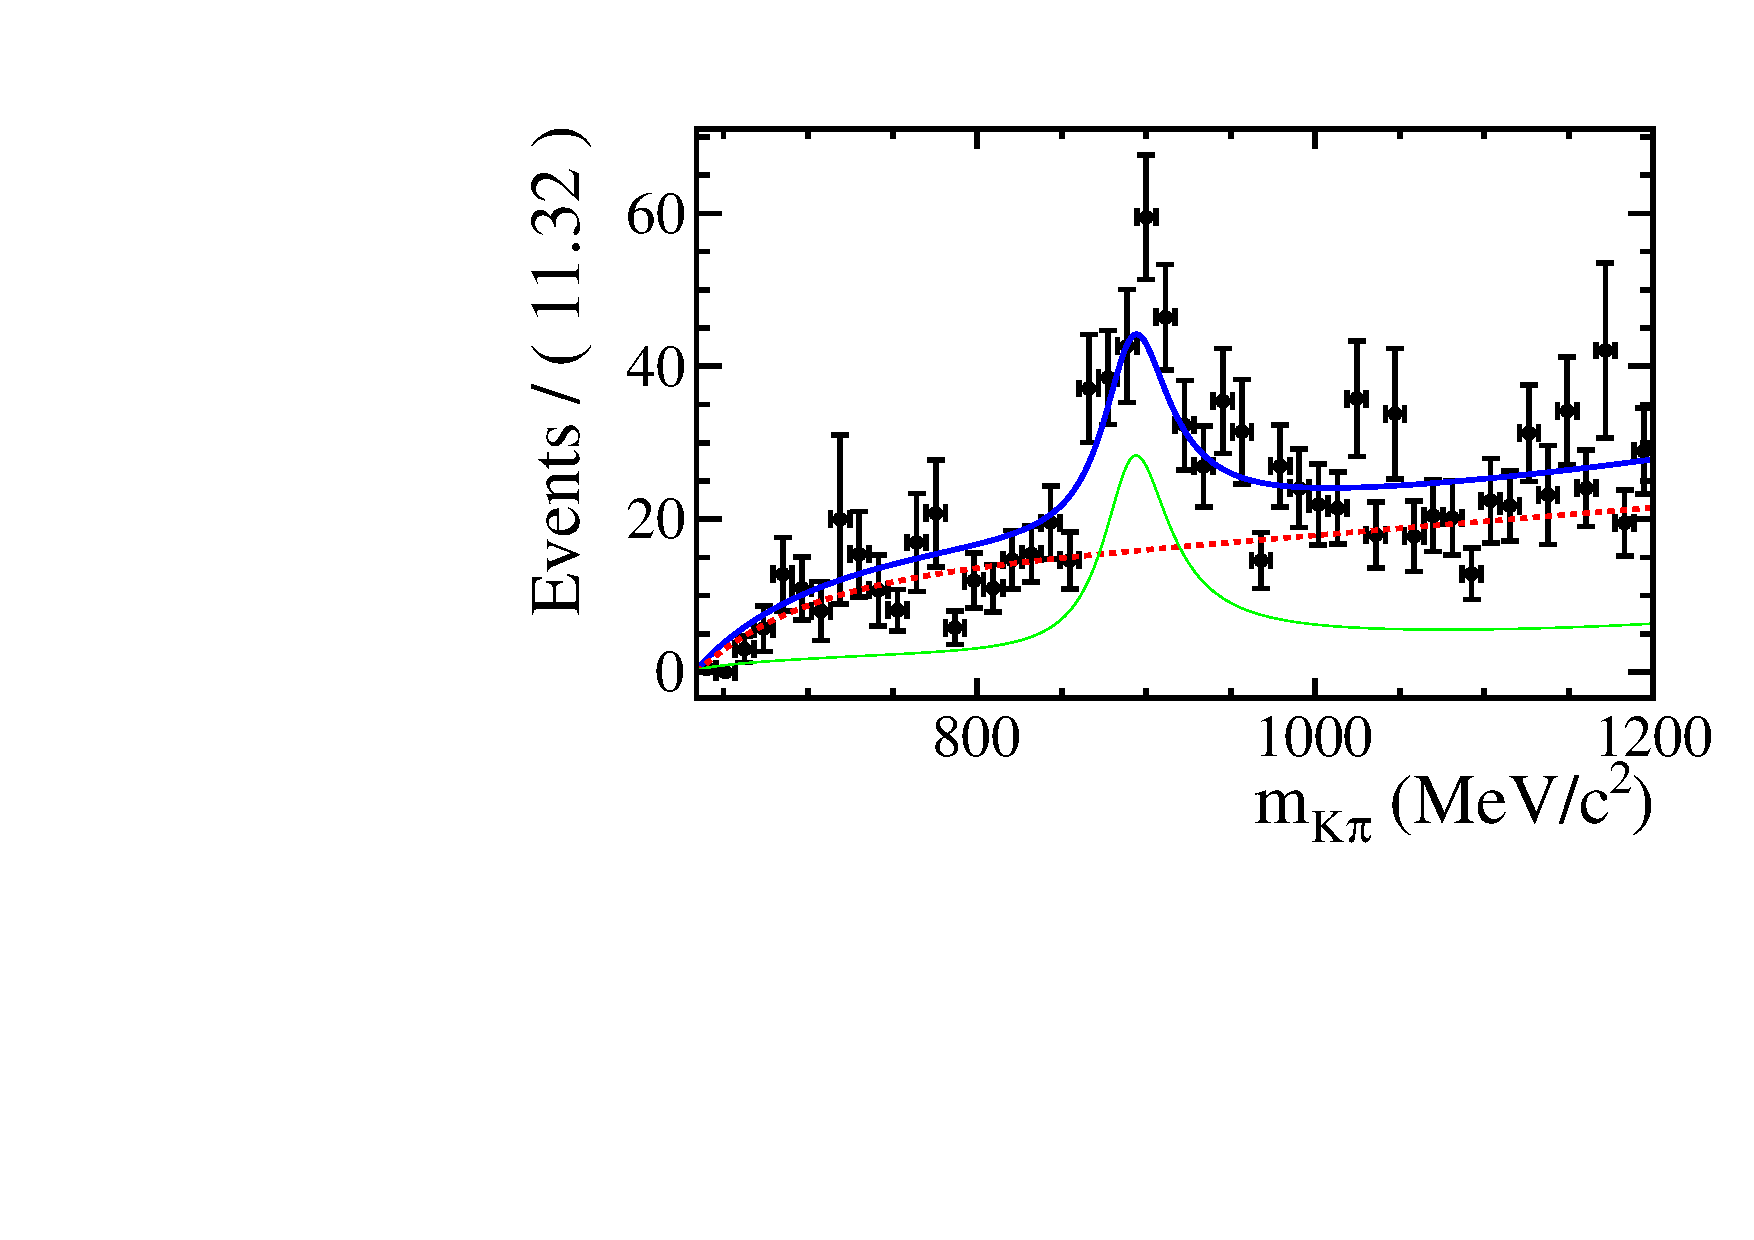
\includegraphics[width=0.48\columnwidth]
{chapter7/figs/fits/lass/fit_kstarmumu_swave_mkpi_range_lass_mkpi_canvas_2.pdf}}
\subfigure{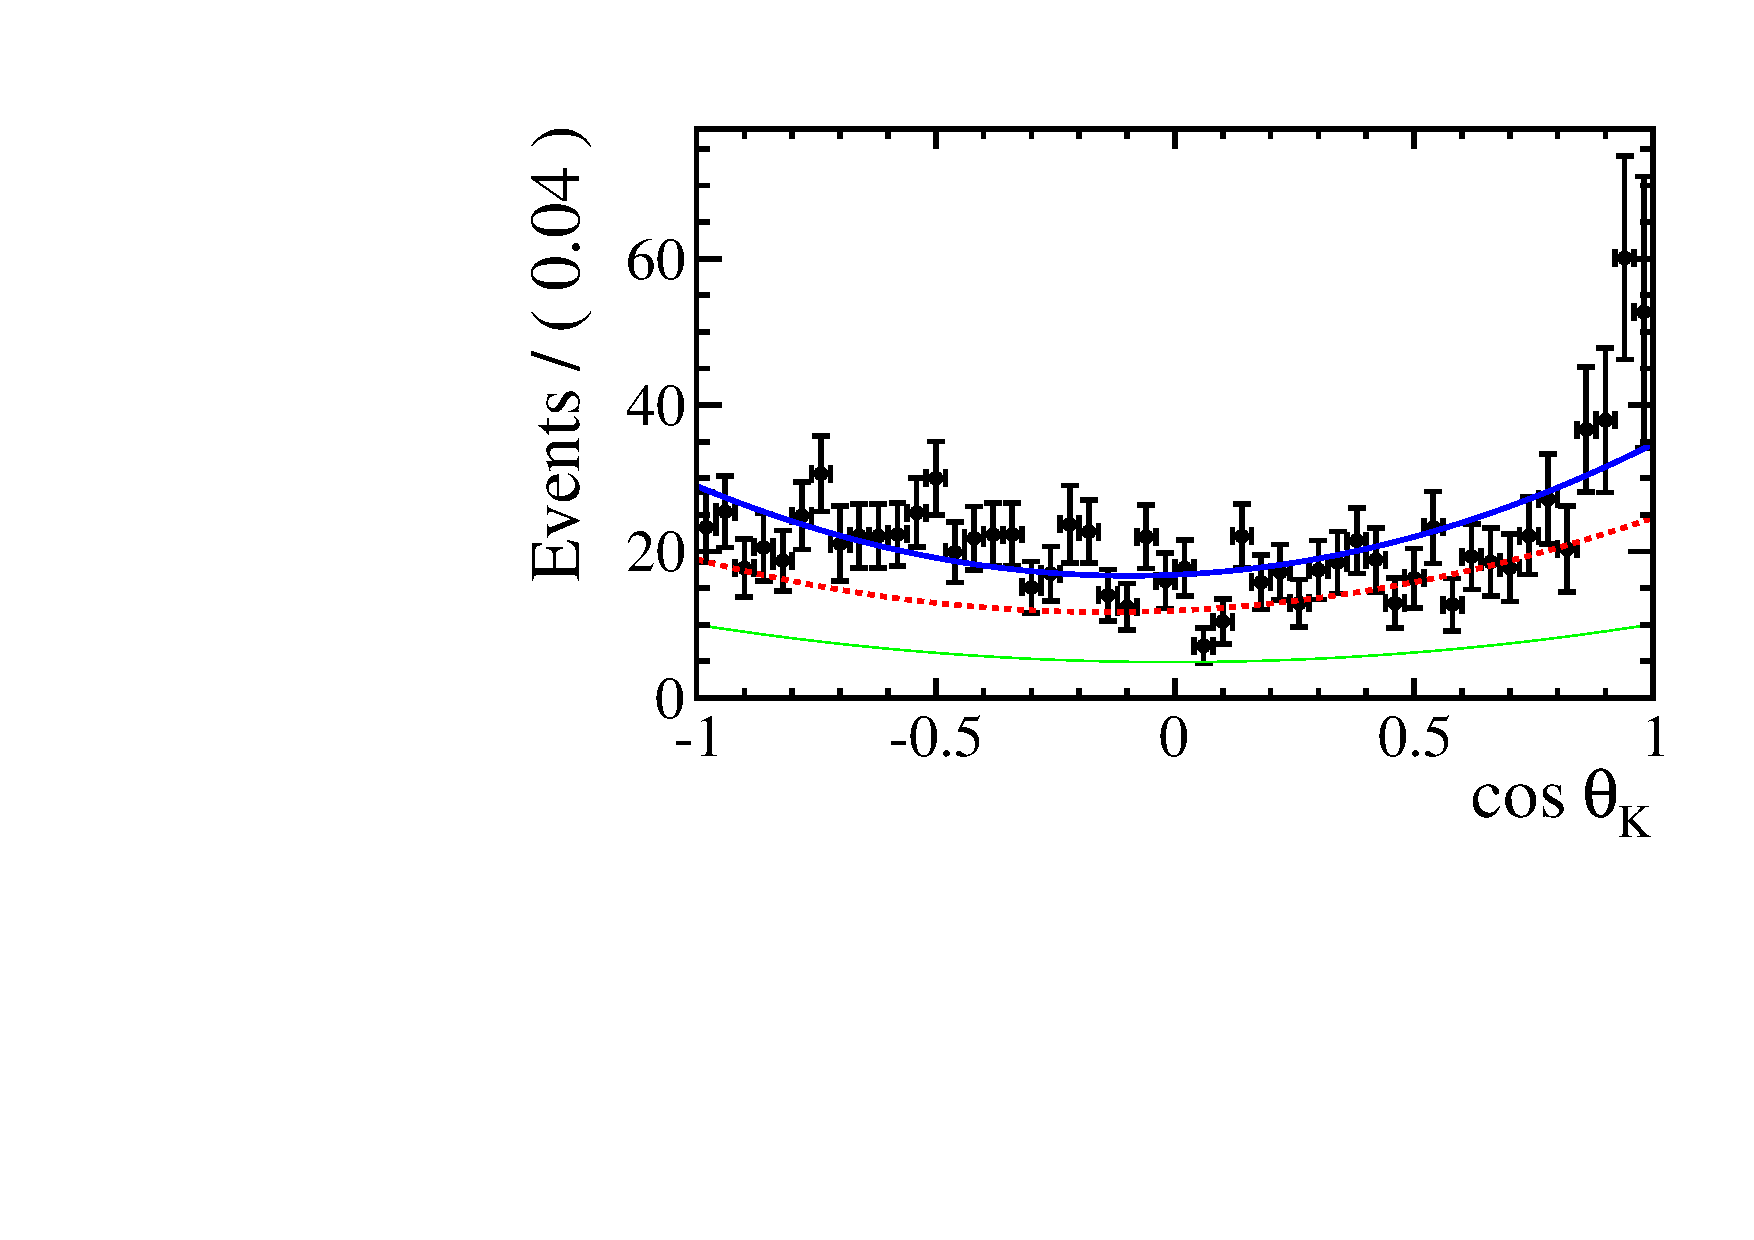
\includegraphics[width=0.48\columnwidth]
{chapter7/figs/fits/lass/fit_kstarmumu_swave_mkpi_range_lass_costhetak_canvas_2.pdf}}
\caption{ The result of the fit to the \qsq region from 4.3 to 8.68 \gevgevcccc. }
\end{figure}

\begin{figure}[tbp]
\centering
\subfigure{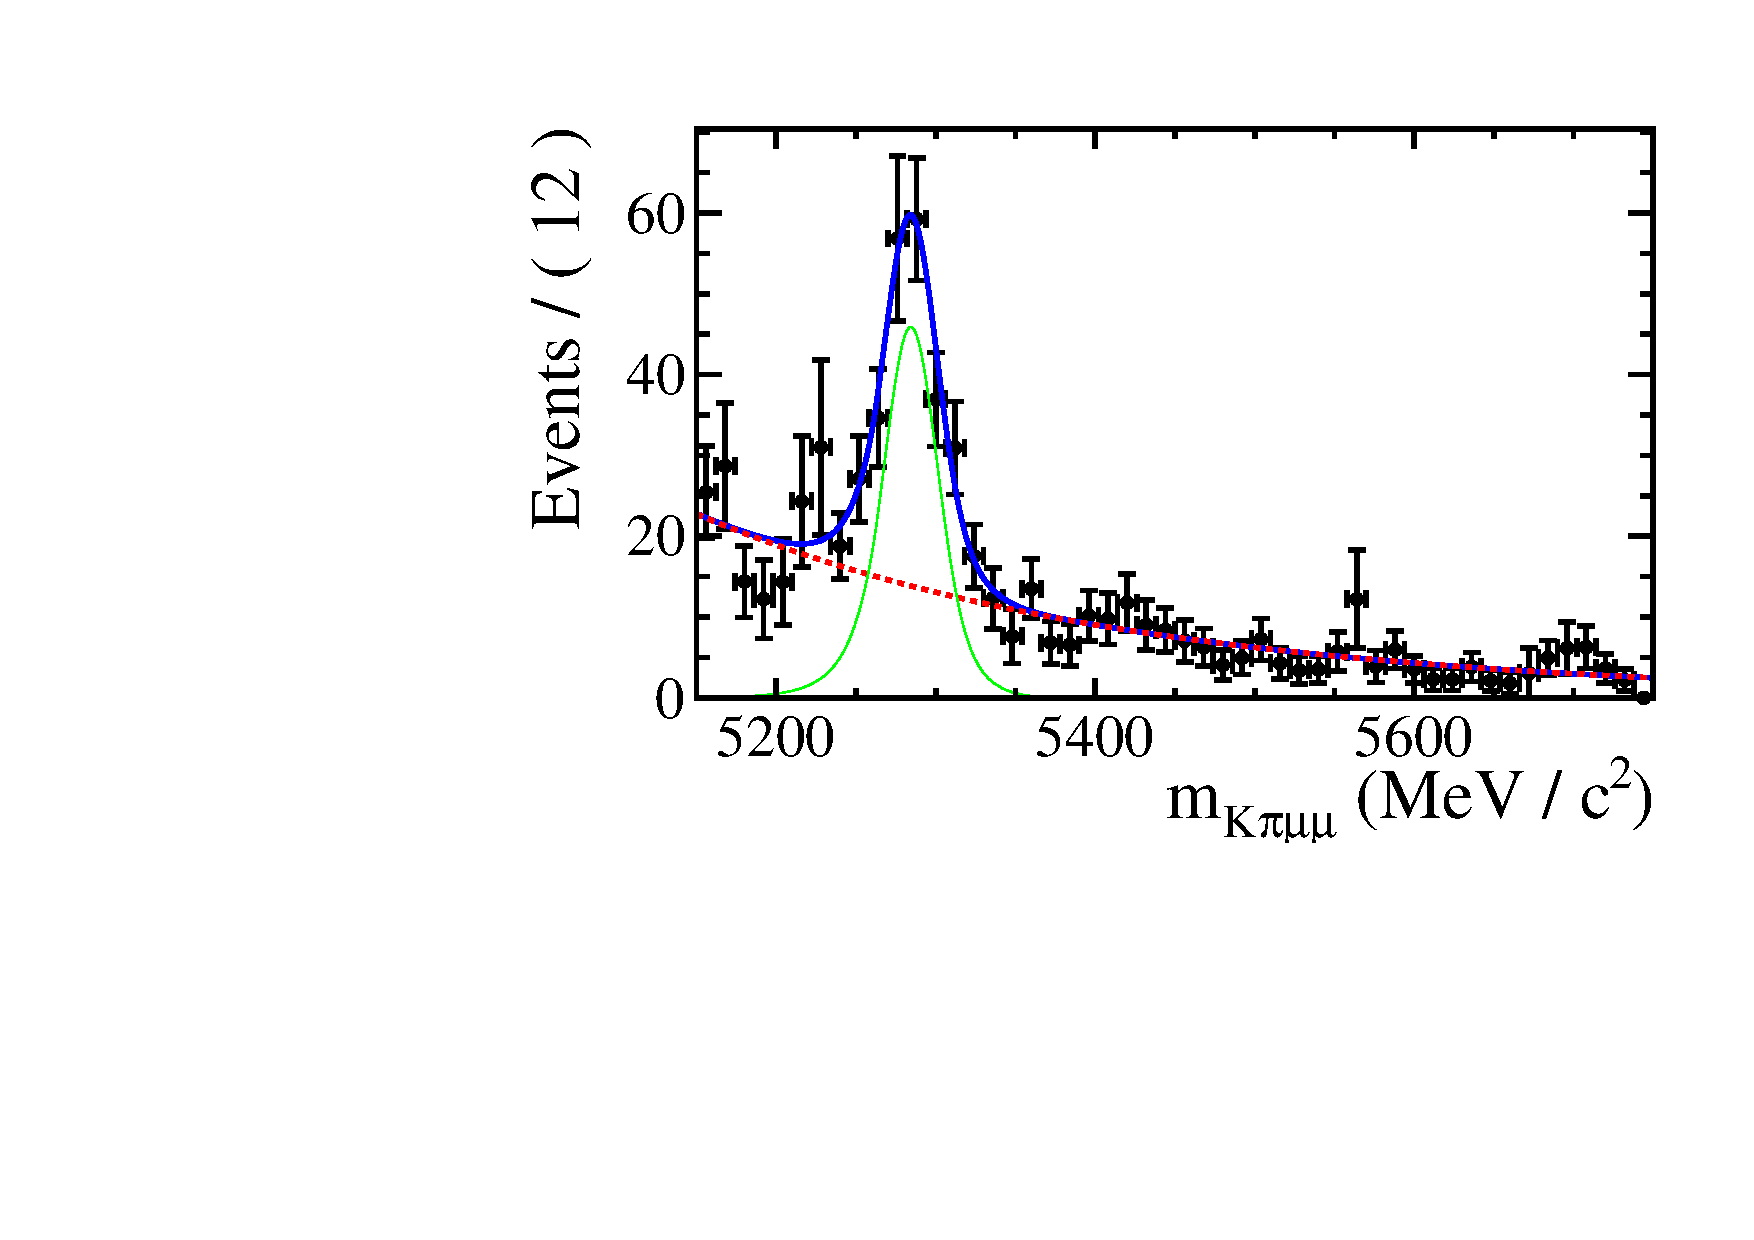
\includegraphics[width=0.48\columnwidth]
{chapter7/figs/fits/lass/fit_kstarmumu_swave_mkpi_range_lass_mass_canvas_3.pdf}}
\subfigure{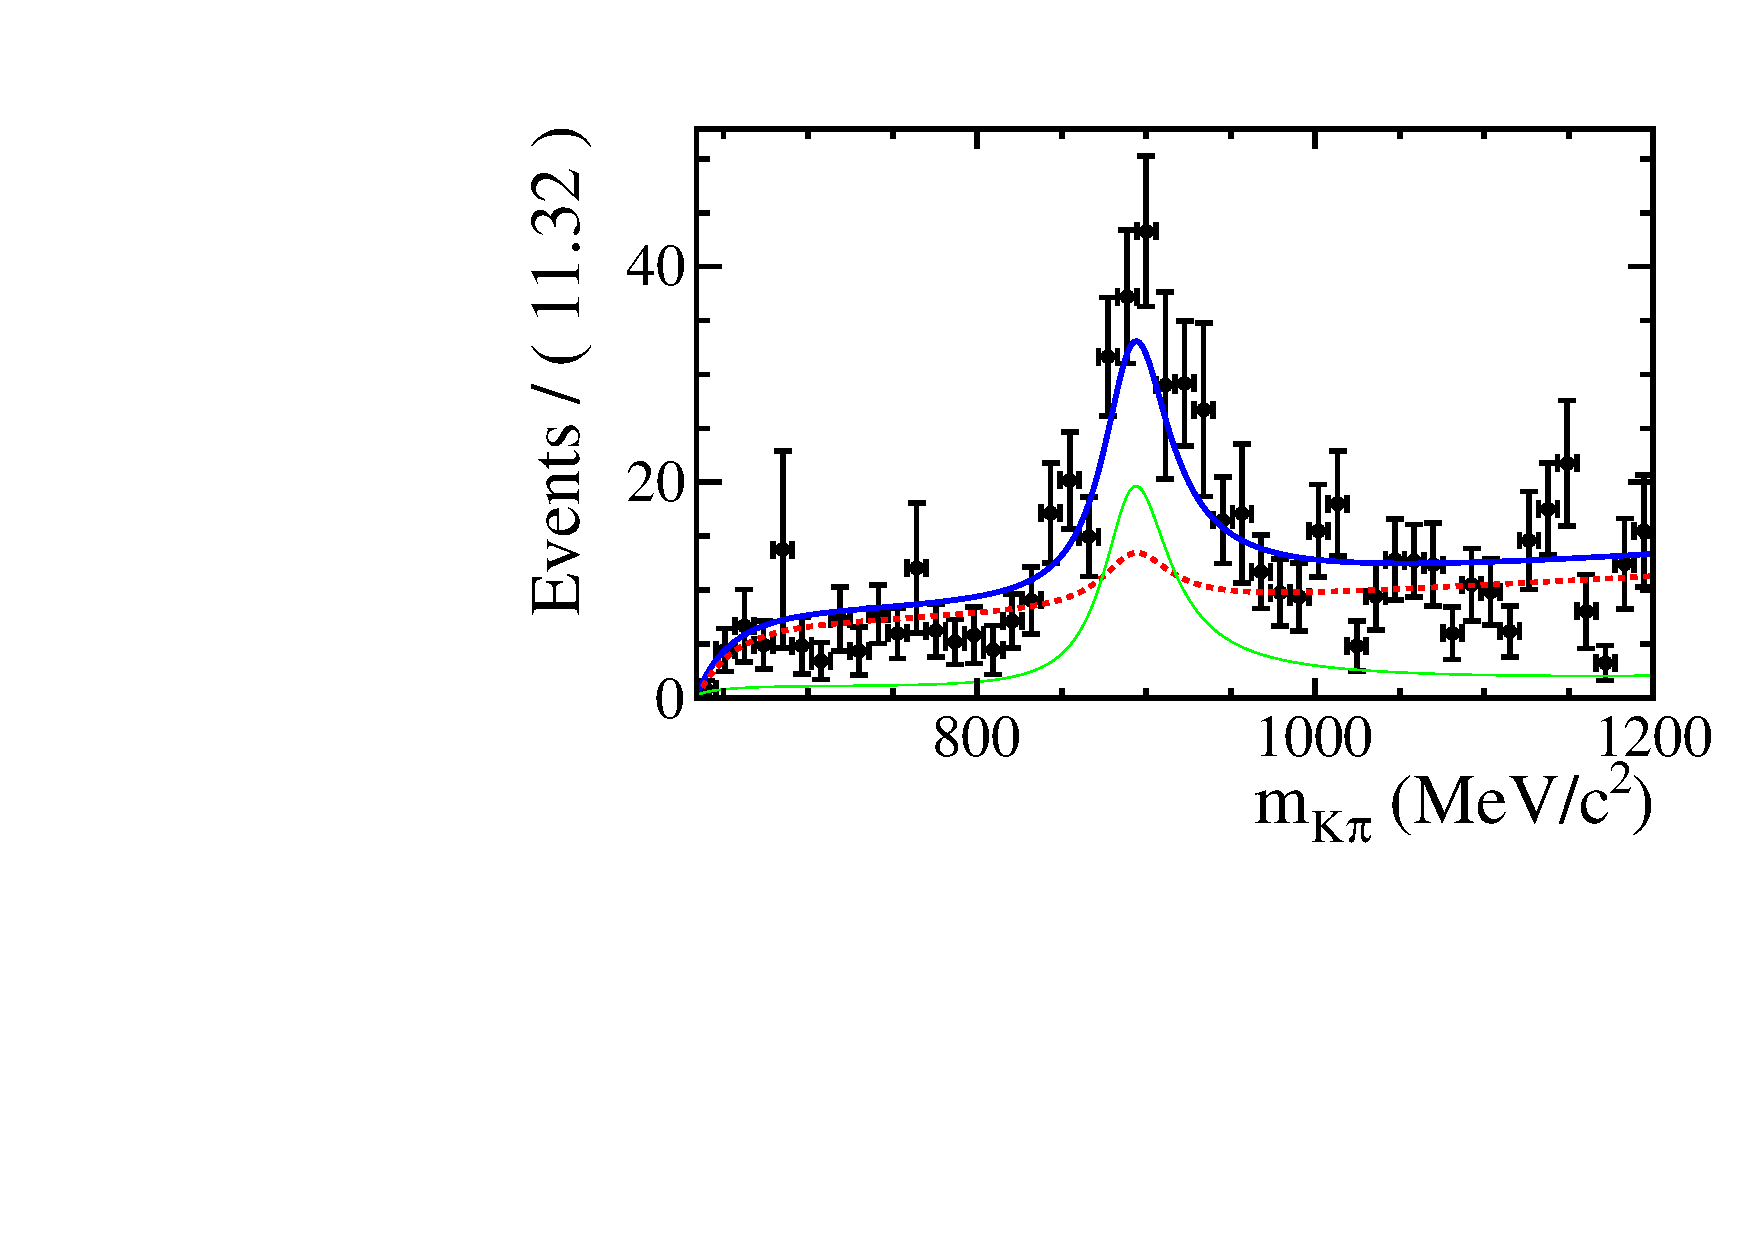
\includegraphics[width=0.48\columnwidth]
{chapter7/figs/fits/lass/fit_kstarmumu_swave_mkpi_range_lass_mkpi_canvas_3.pdf}}
\subfigure{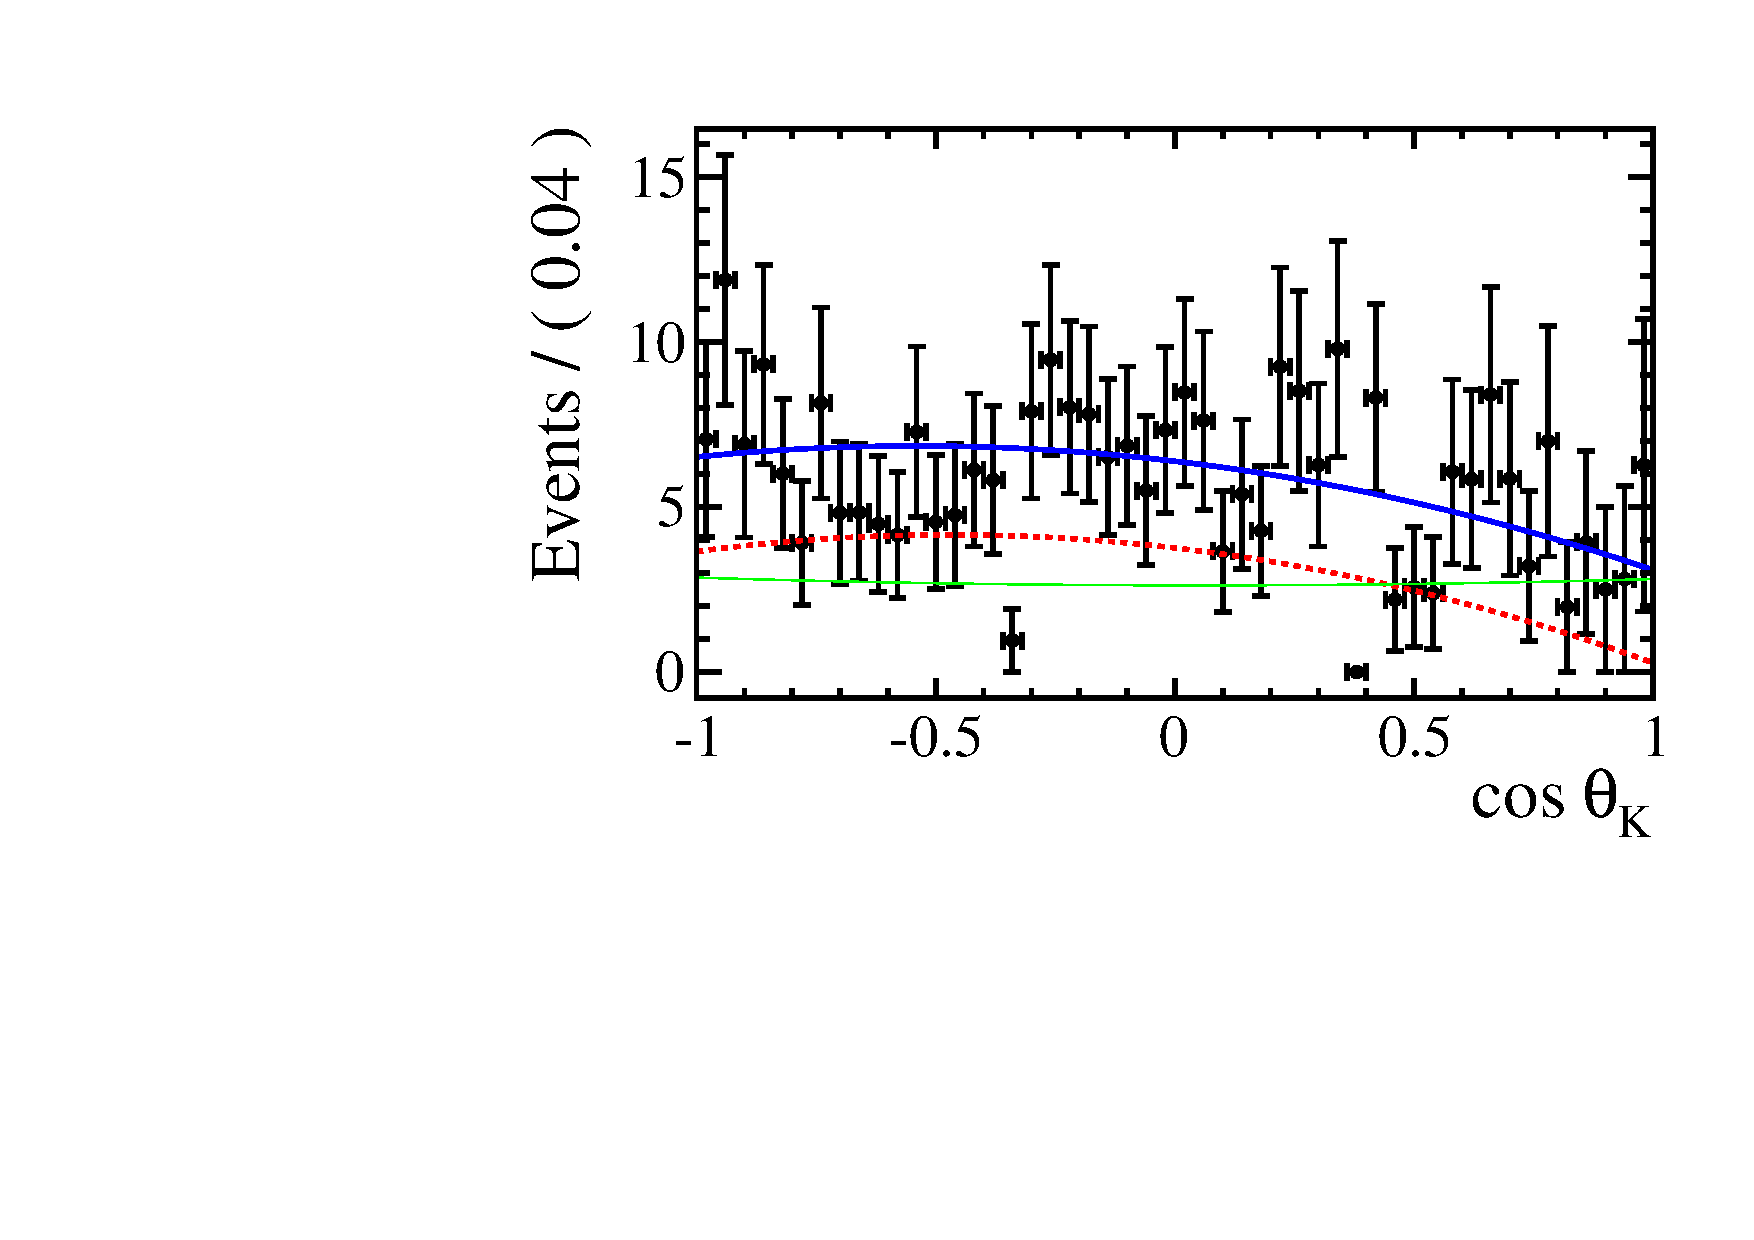
\includegraphics[width=0.48\columnwidth]
{chapter7/figs/fits/lass/fit_kstarmumu_swave_mkpi_range_lass_costhetak_canvas_4.pdf}}
\caption{ The result of the fit to the \qsq region from 10.06 to 12.9 \gevgevcccc. }
\end{figure}

\begin{figure}[tbp]
\centering
\subfigure{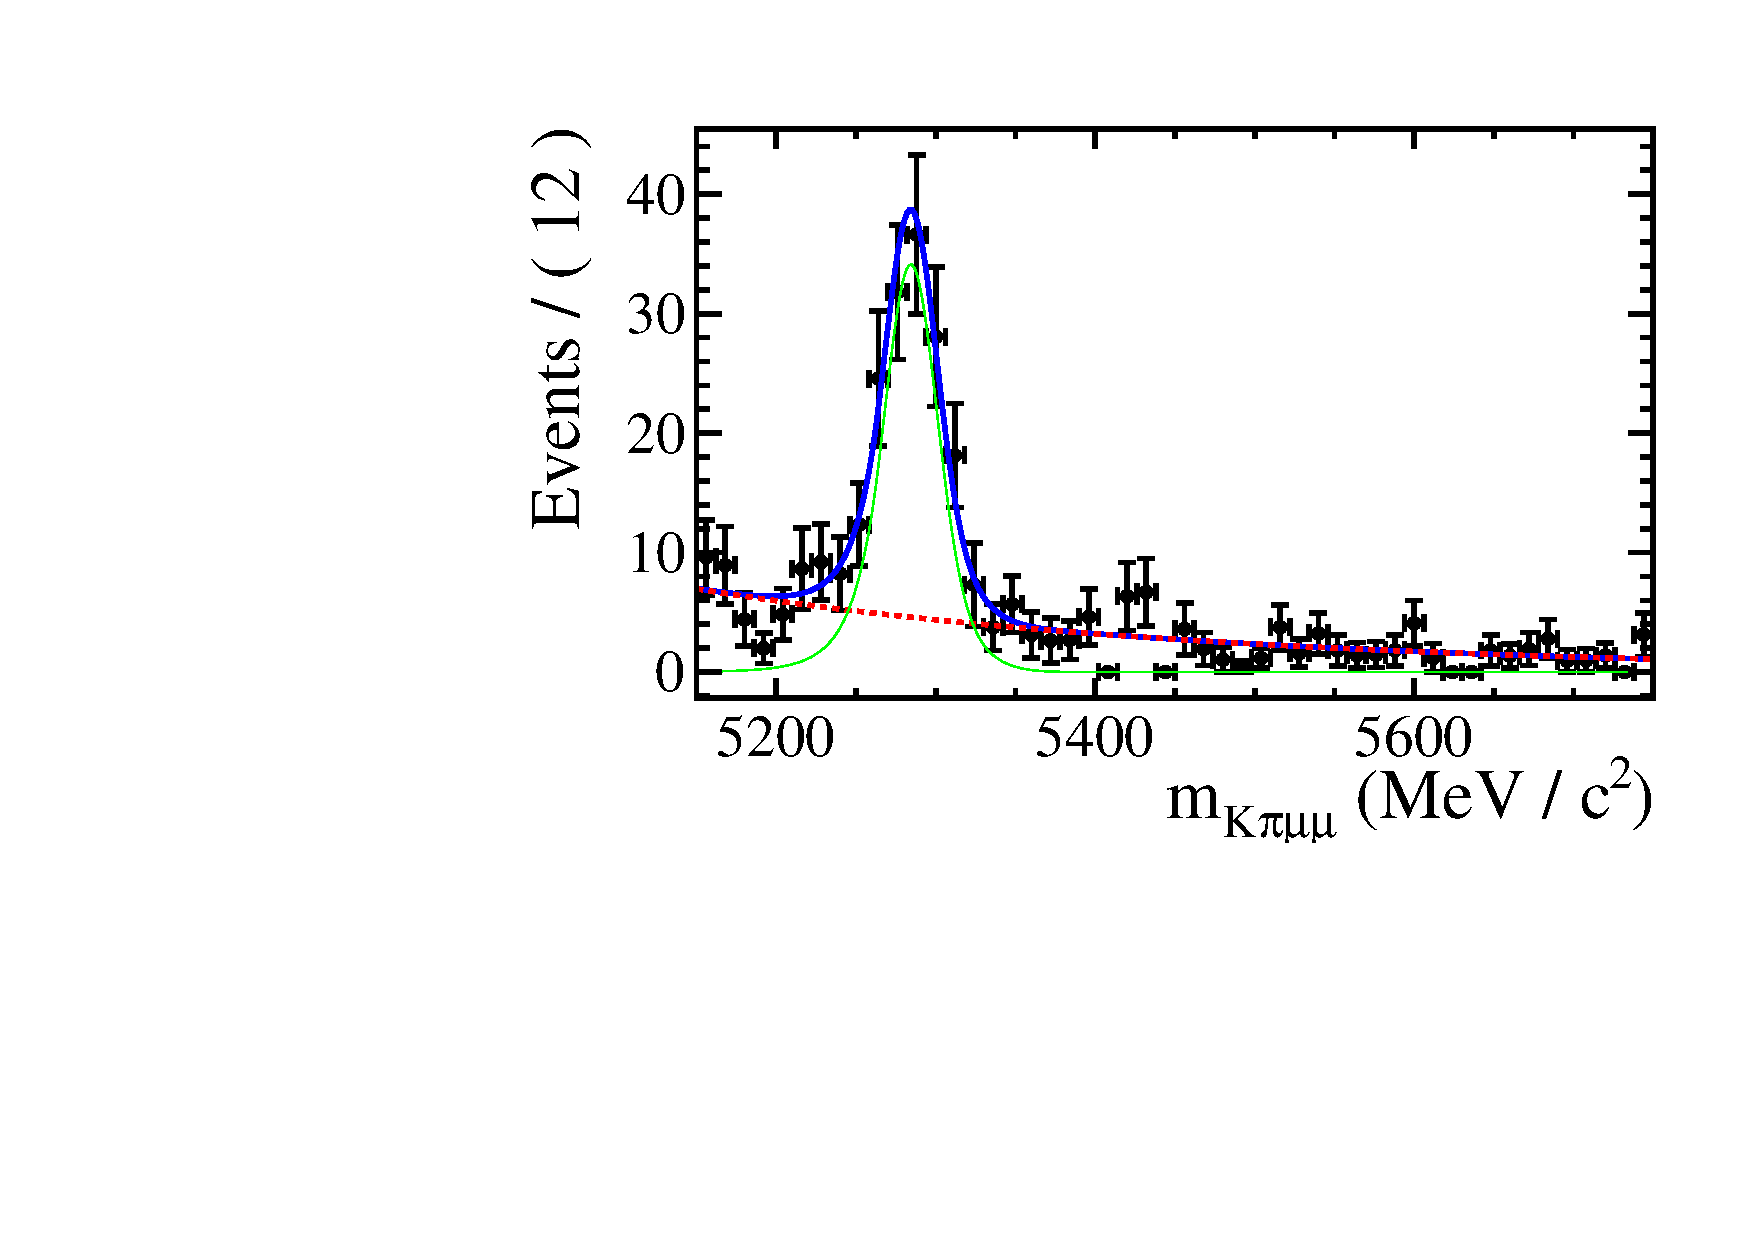
\includegraphics[width=0.48\columnwidth]
{chapter7/figs/fits/lass/fit_kstarmumu_swave_mkpi_range_lass_mass_canvas_4.pdf}}
\subfigure{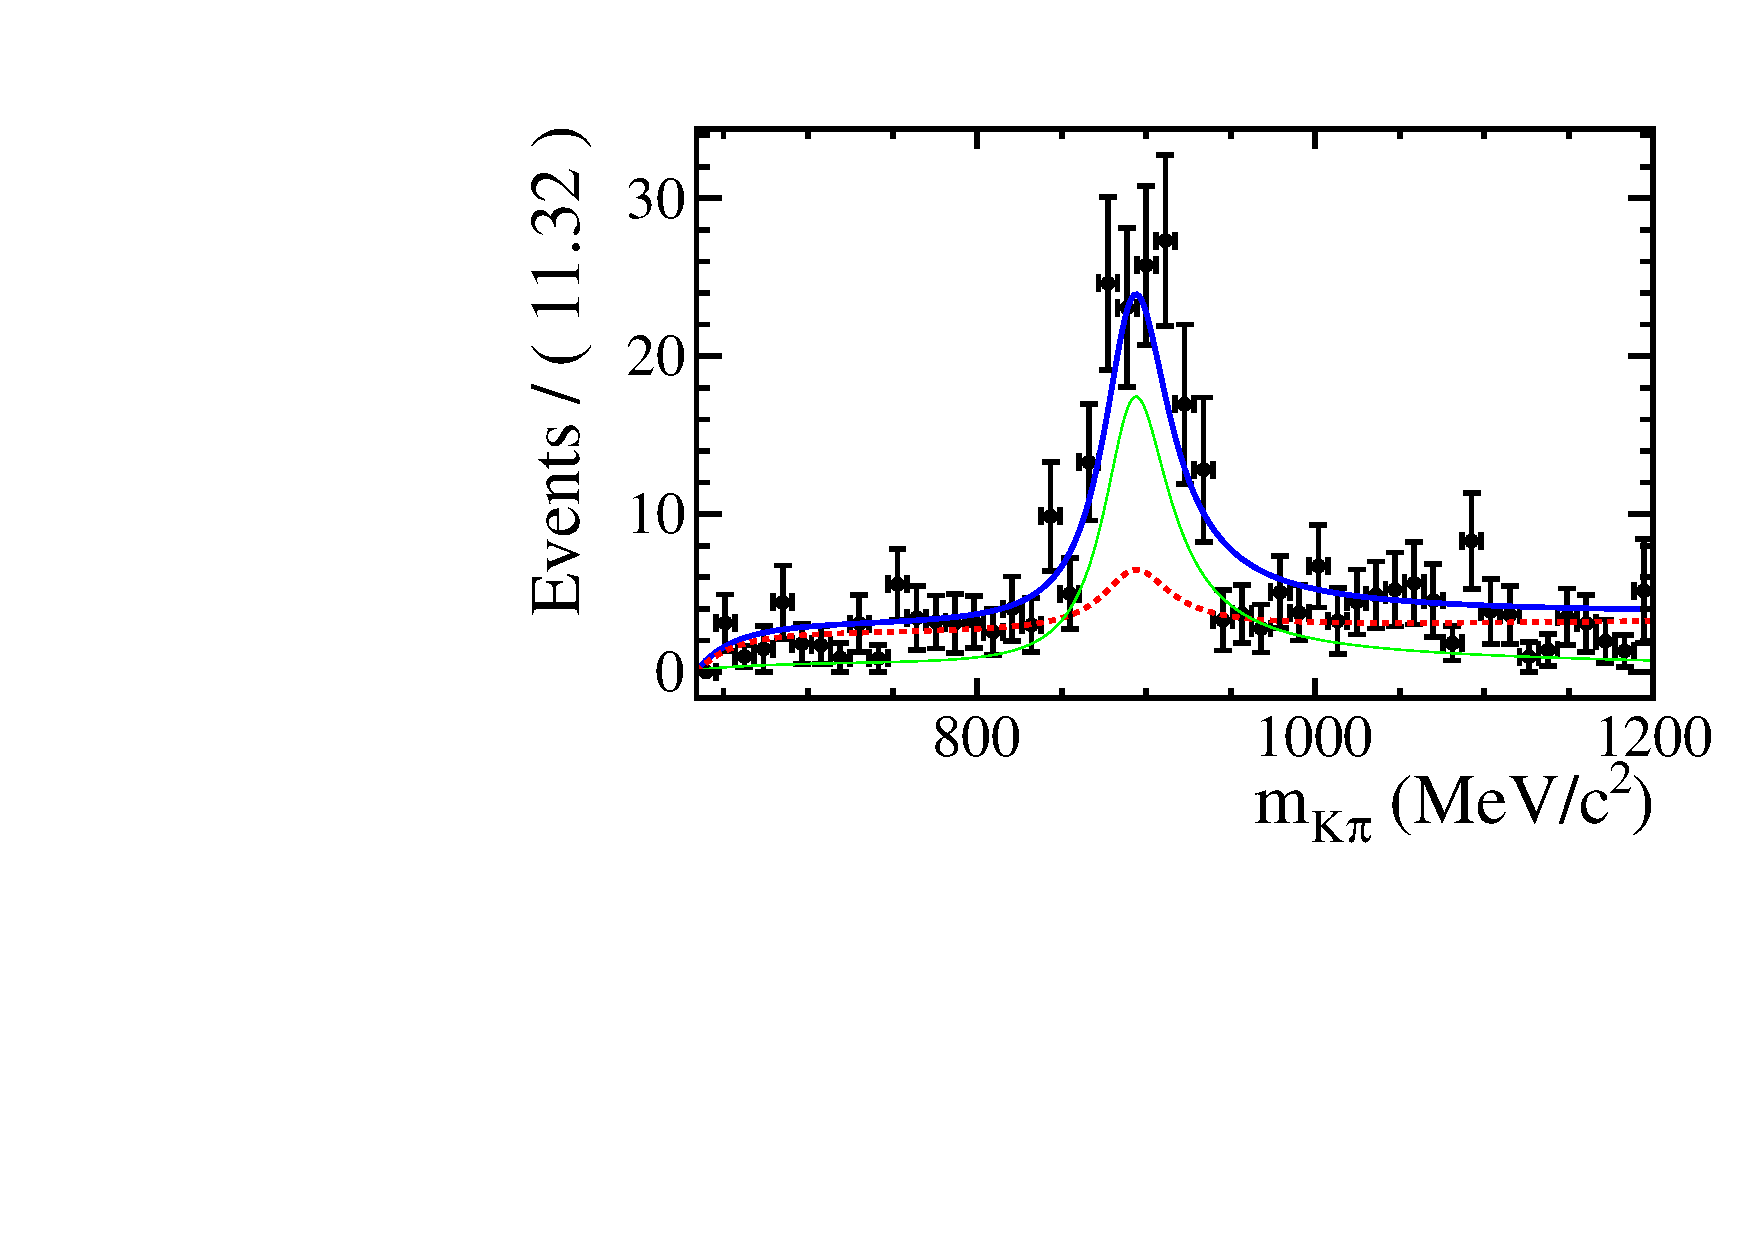
\includegraphics[width=0.48\columnwidth]
{chapter7/figs/fits/lass/fit_kstarmumu_swave_mkpi_range_lass_mkpi_canvas_4.pdf}}
\subfigure{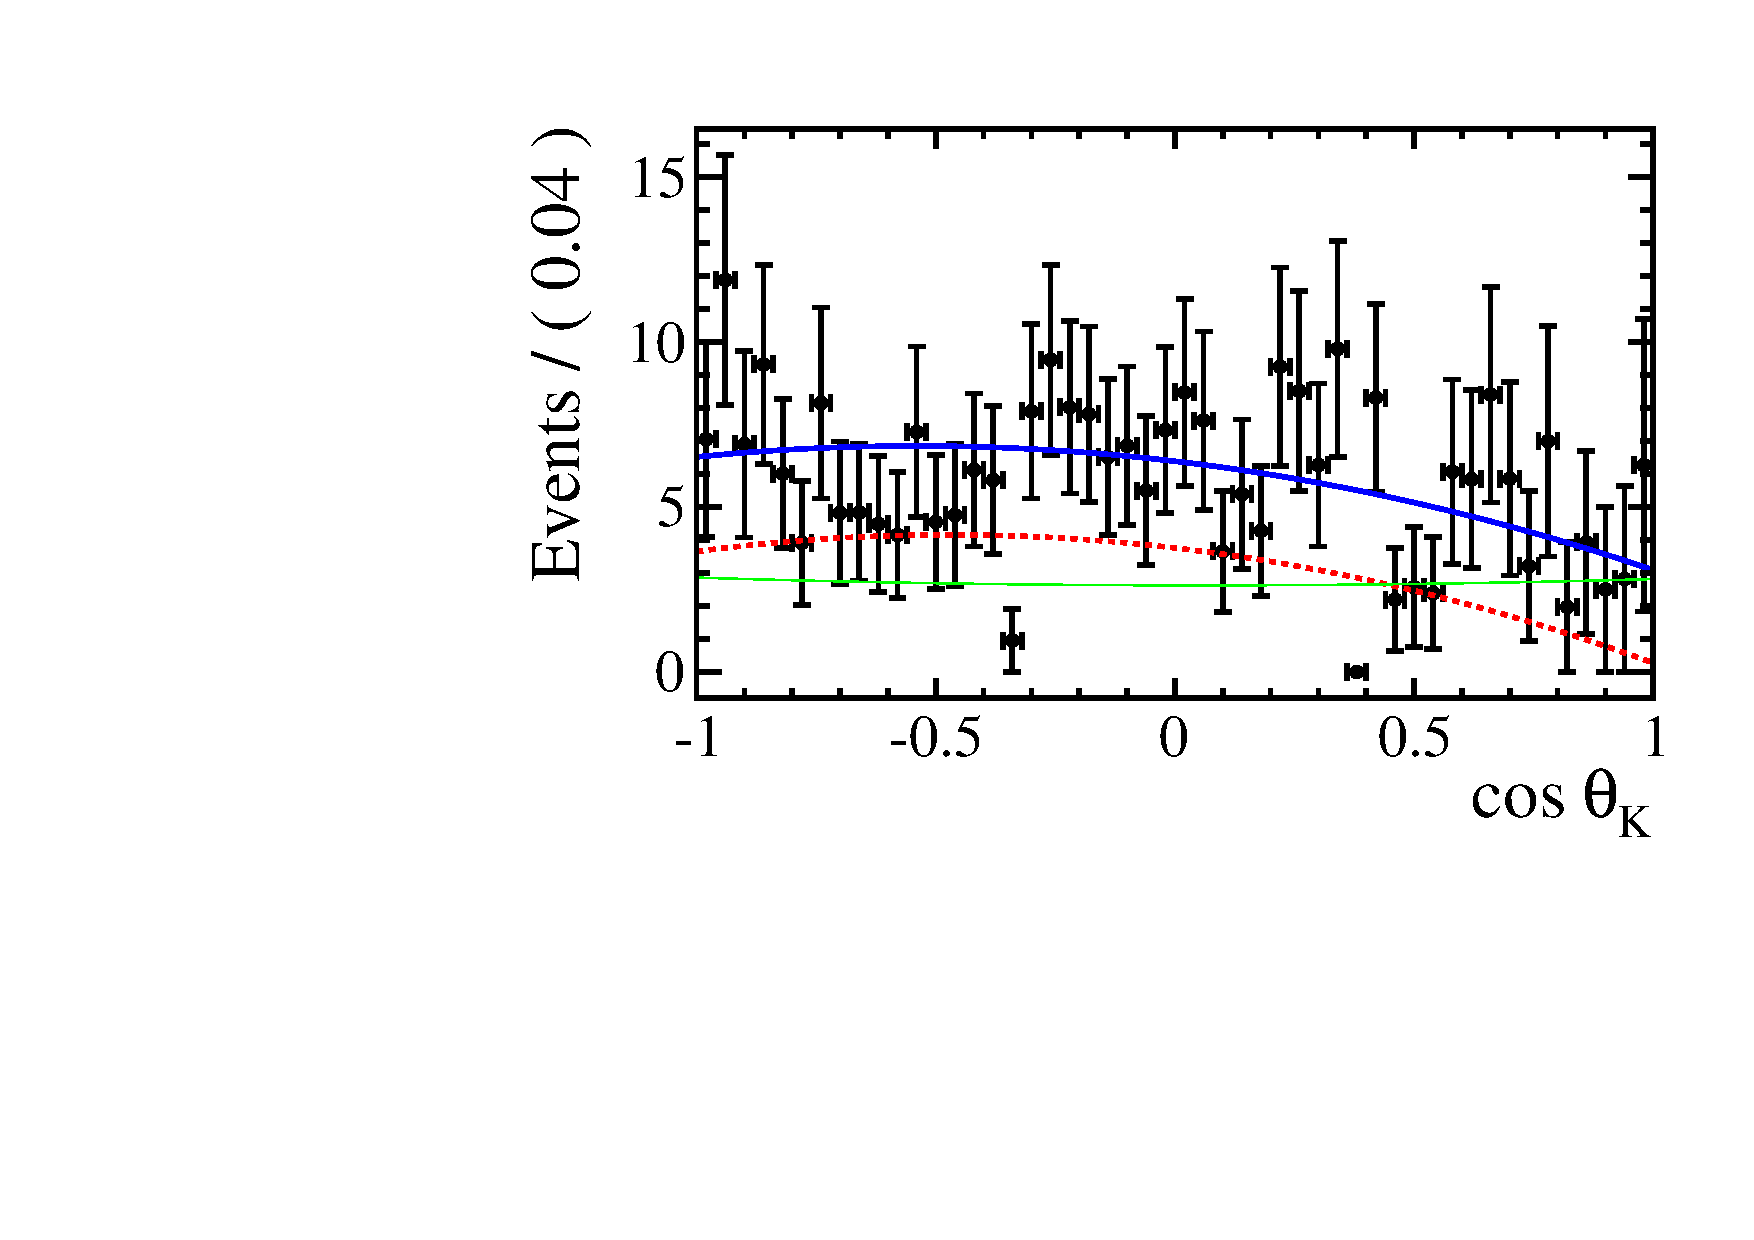
\includegraphics[width=0.48\columnwidth]
{chapter7/figs/fits/lass/fit_kstarmumu_swave_mkpi_range_lass_costhetak_canvas_4.pdf}}
\caption{ The result of the fit to the \qsq region from 14 to 16 \gevgevcccc. }
\end{figure}

\begin{figure}[tbp]
\centering
\subfigure{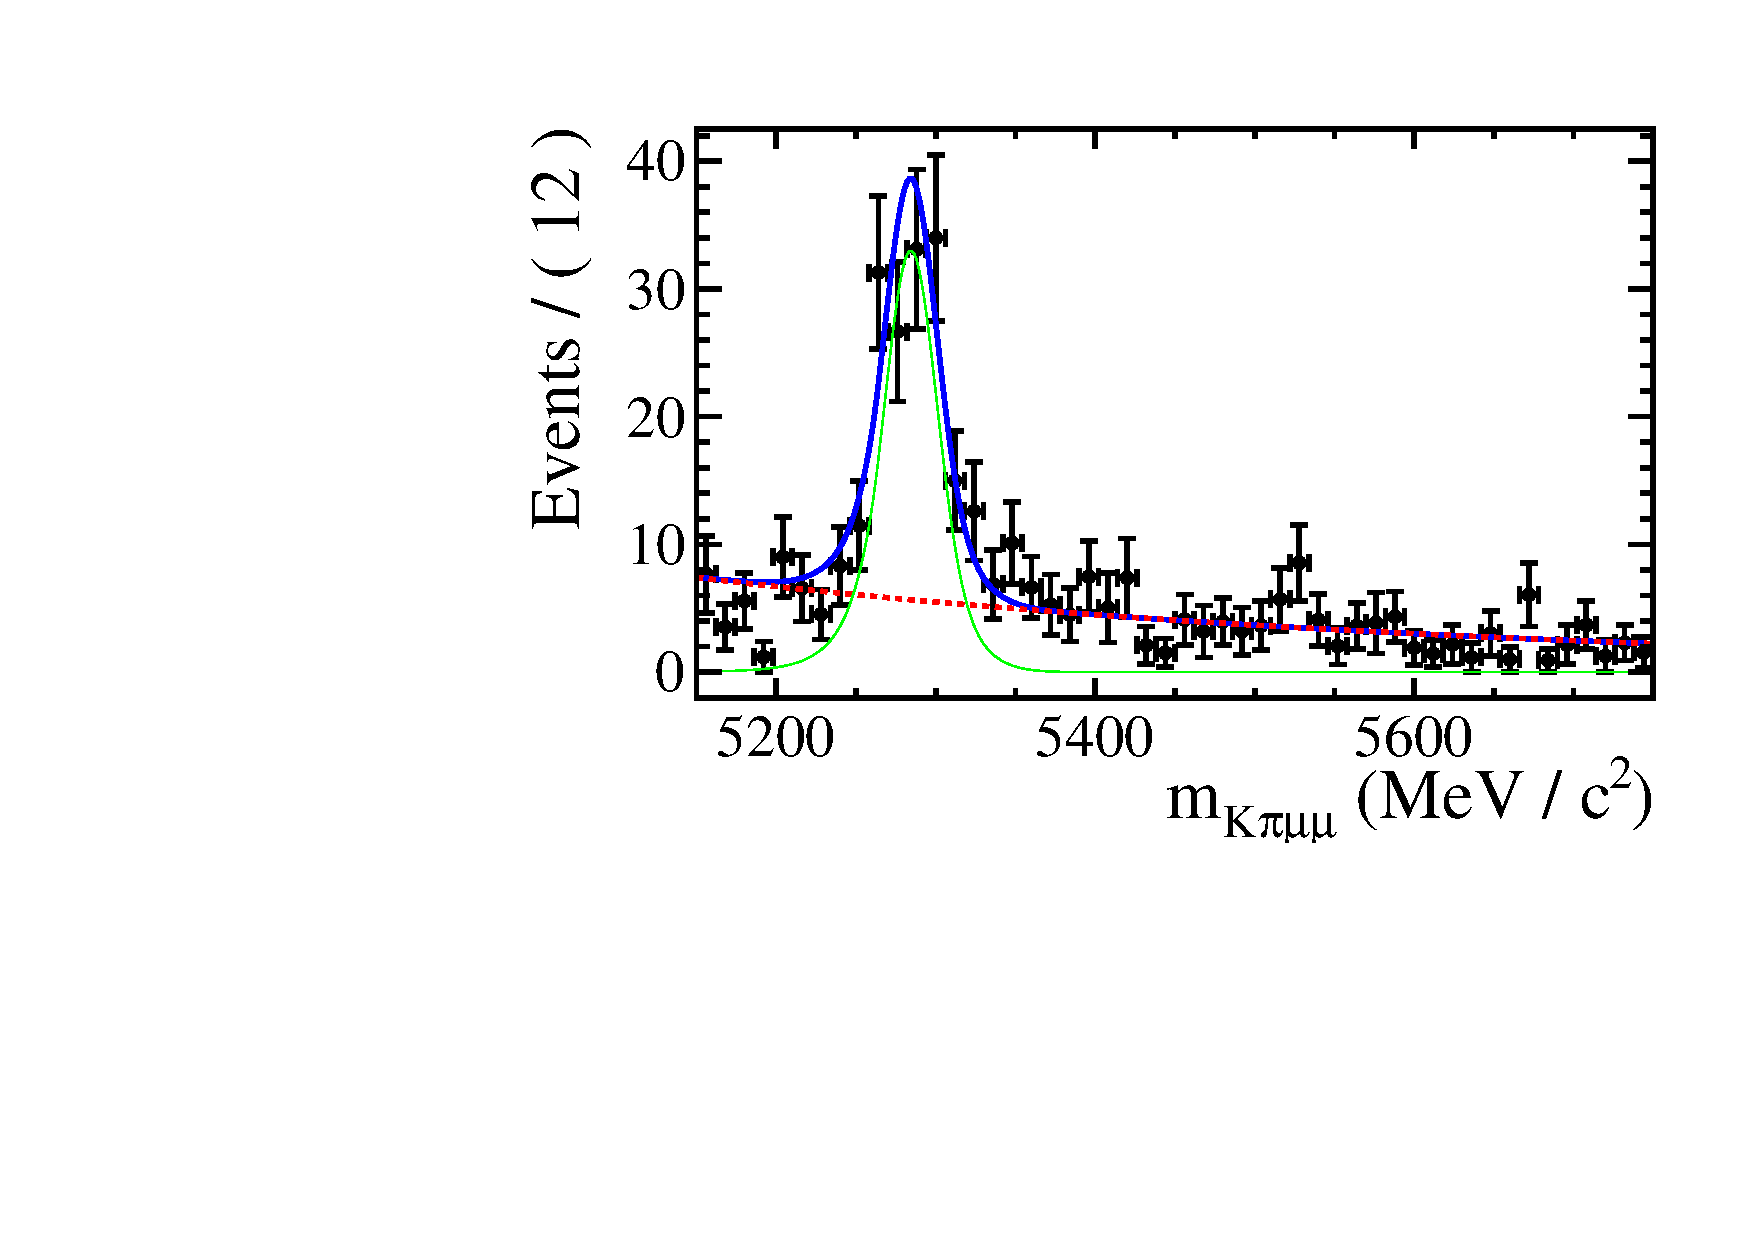
\includegraphics[width=0.48\columnwidth]
{chapter7/figs/fits/lass/fit_kstarmumu_swave_mkpi_range_lass_mass_canvas_5.pdf}}
\subfigure{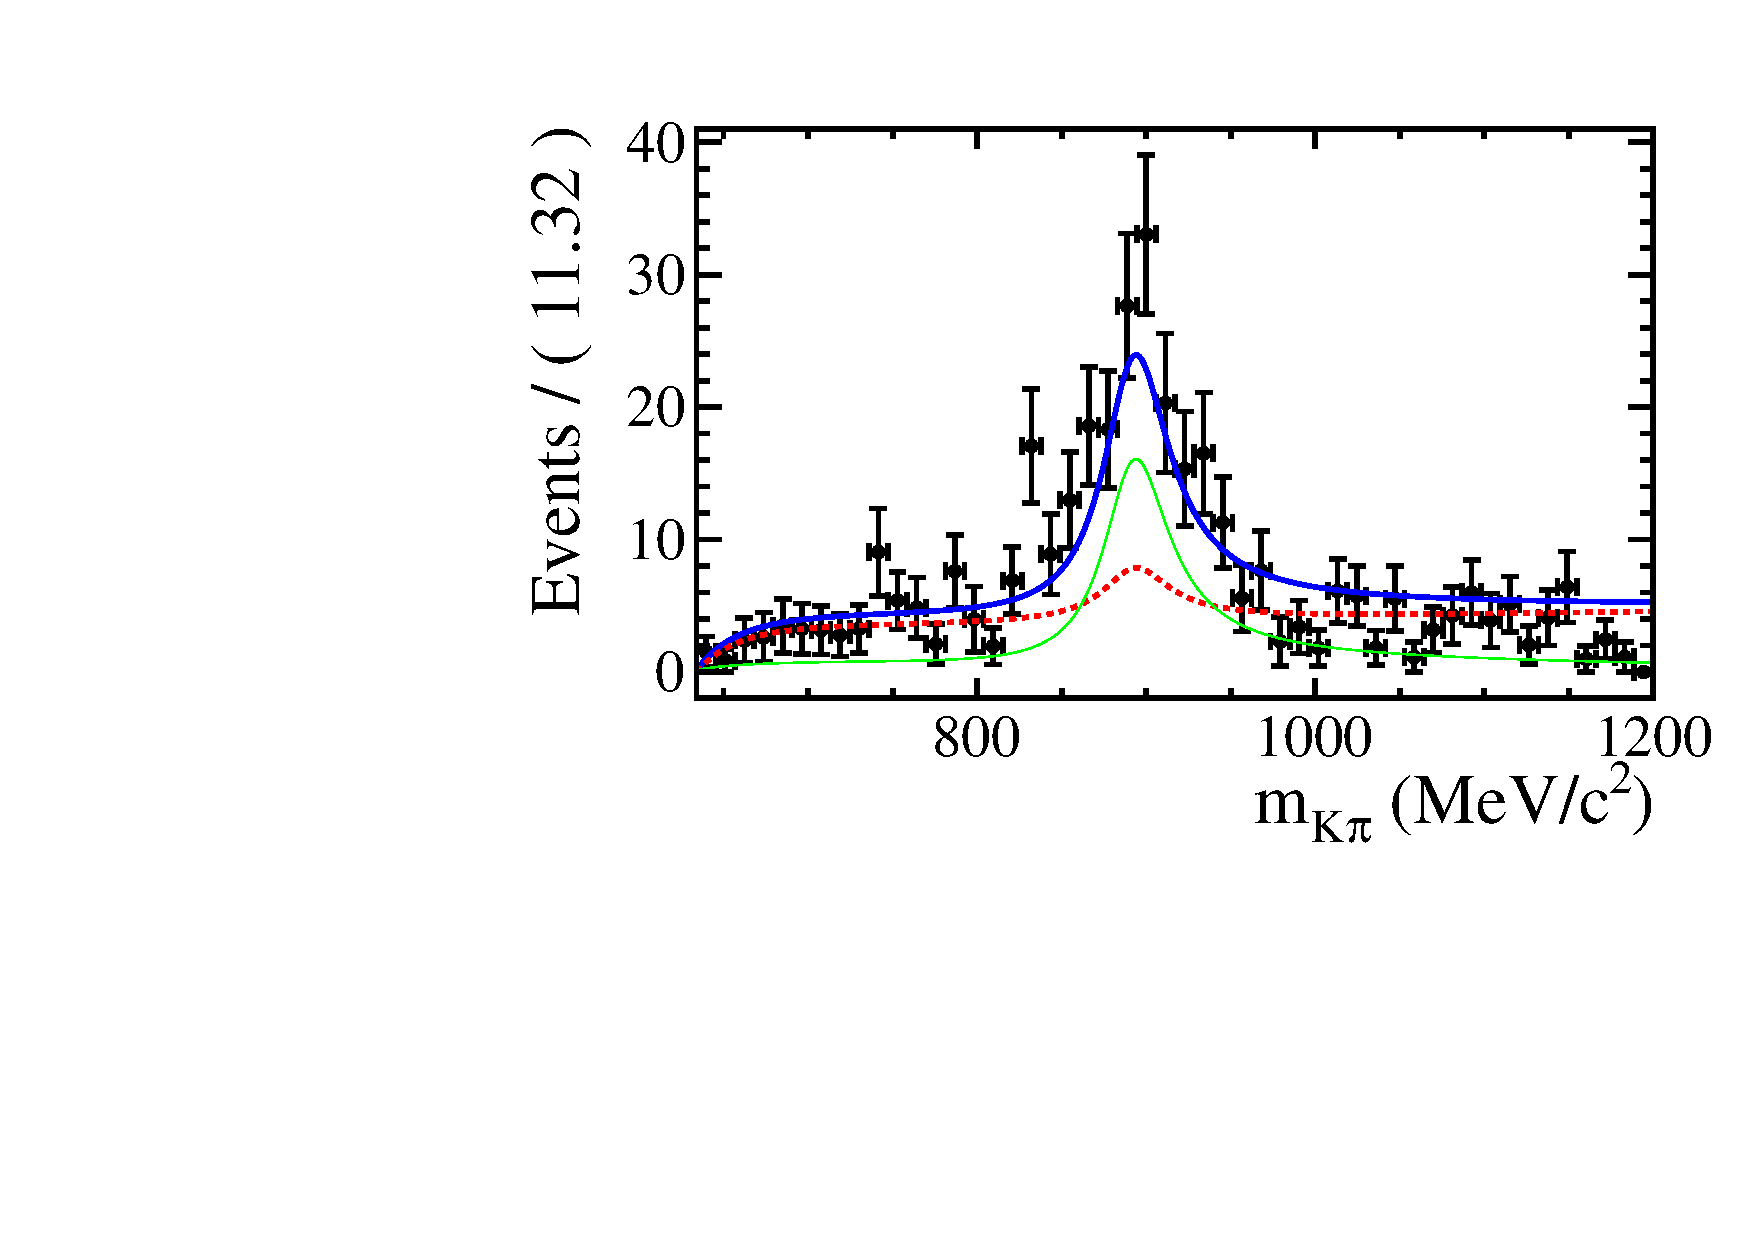
\includegraphics[width=0.48\columnwidth]
{chapter7/figs/fits/lass/fit_kstarmumu_swave_mkpi_range_lass_mkpi_canvas_5.pdf}}
\subfigure{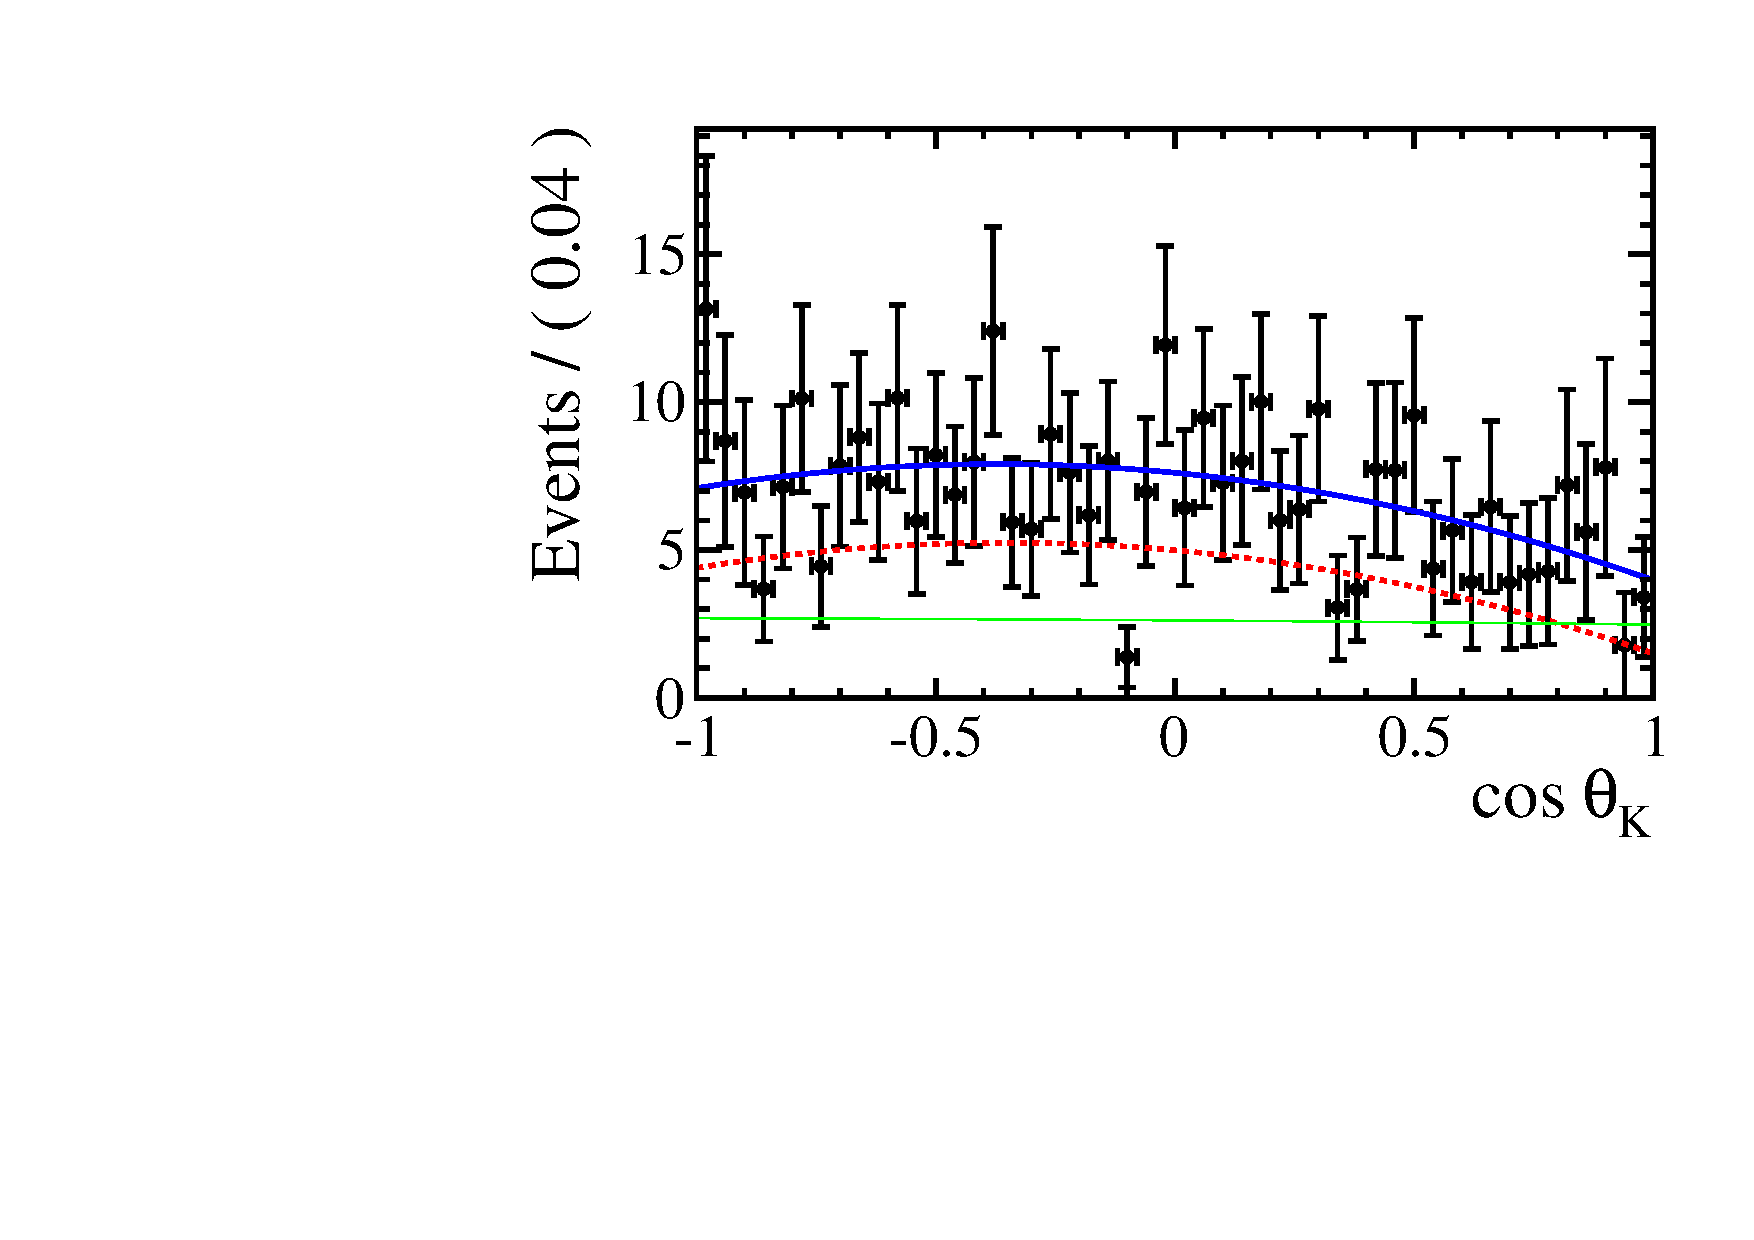
\includegraphics[width=0.48\columnwidth]
{chapter7/figs/fits/lass/fit_kstarmumu_swave_mkpi_range_lass_costhetak_canvas_5.pdf}}
\caption{ The result of the fit to the \qsq region from 16 to 19 \gevgevcccc. }
\end{figure}

\begin{figure}[tbp]
\centering
\subfigure{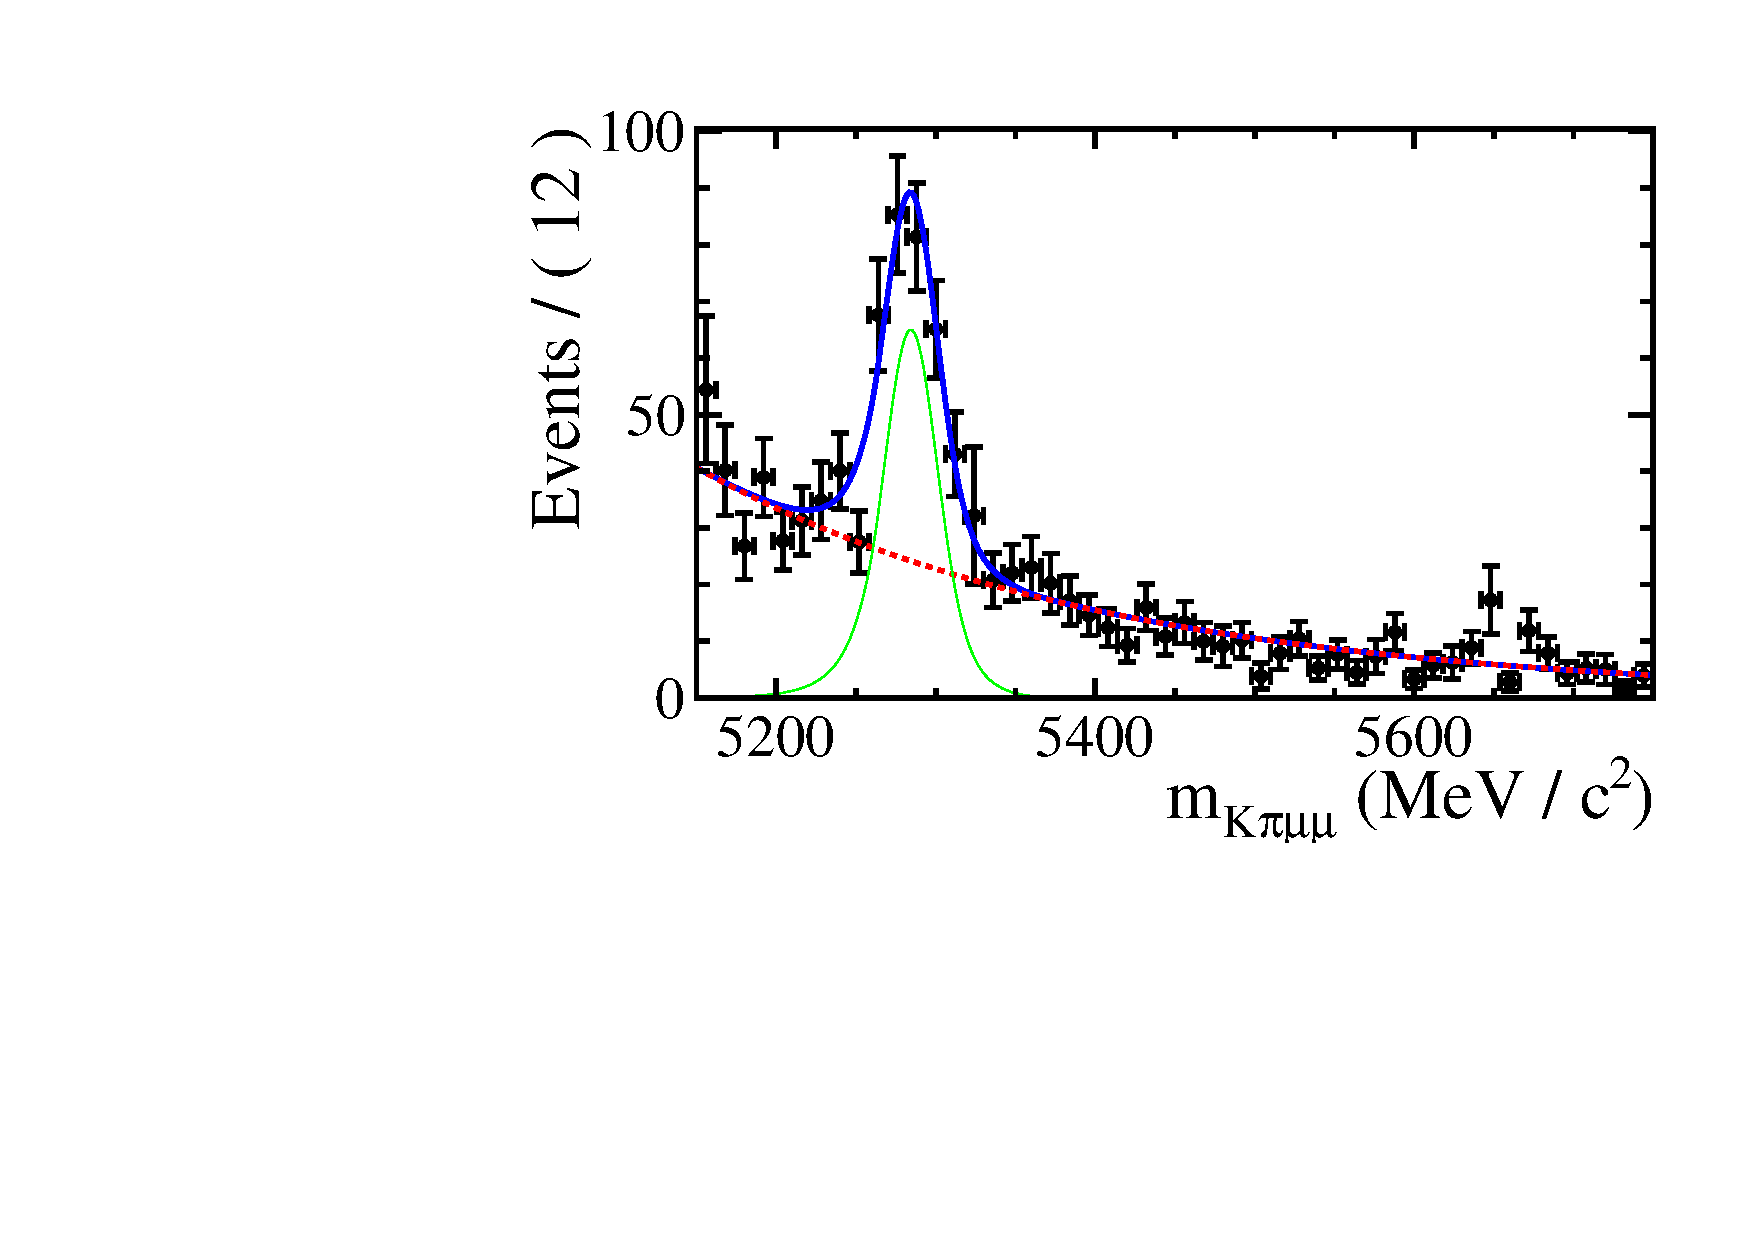
\includegraphics[width=0.48\columnwidth]
{chapter7/figs/fits/lass/fit_kstarmumu_swave_mkpi_range_lass_mass_canvas_6.pdf}}
\subfigure{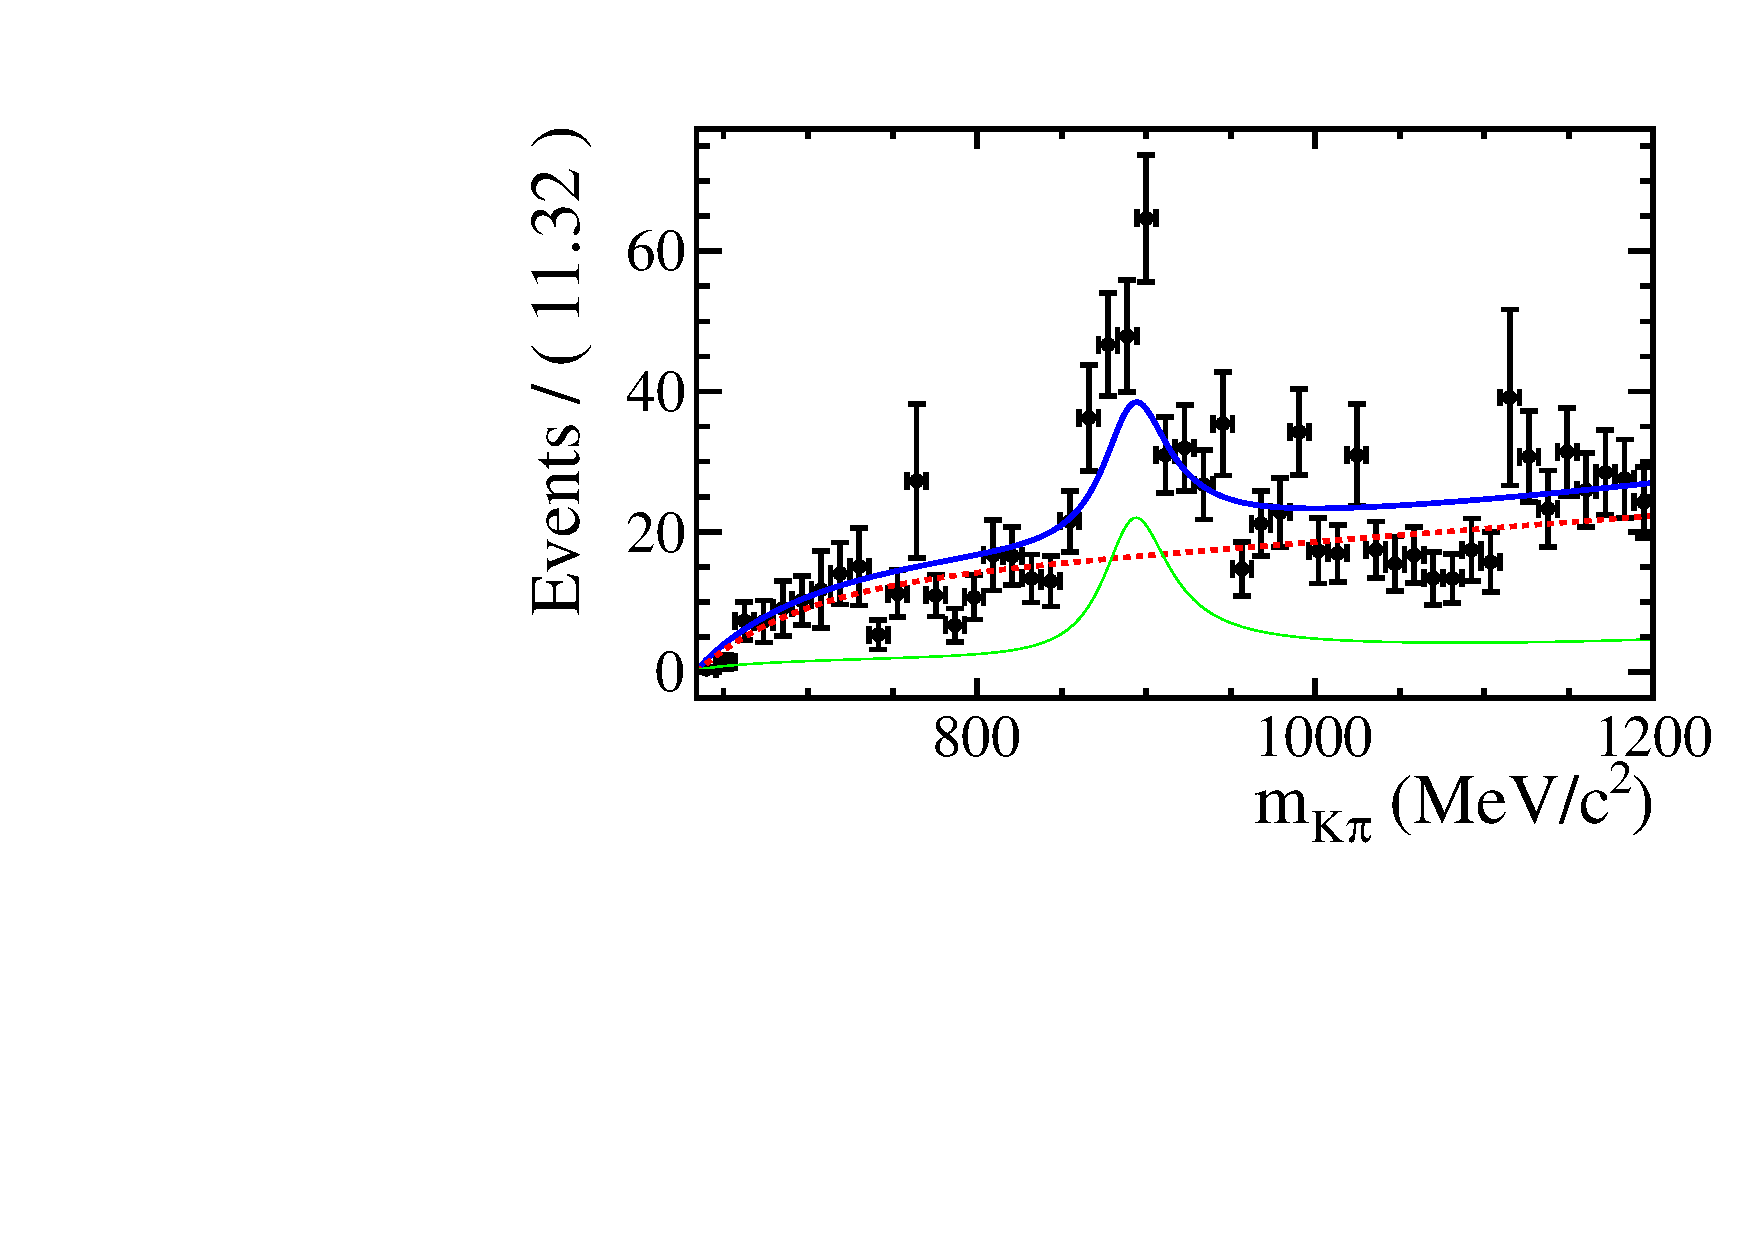
\includegraphics[width=0.48\columnwidth]
{chapter7/figs/fits/lass/fit_kstarmumu_swave_mkpi_range_lass_mkpi_canvas_6.pdf}}
\subfigure{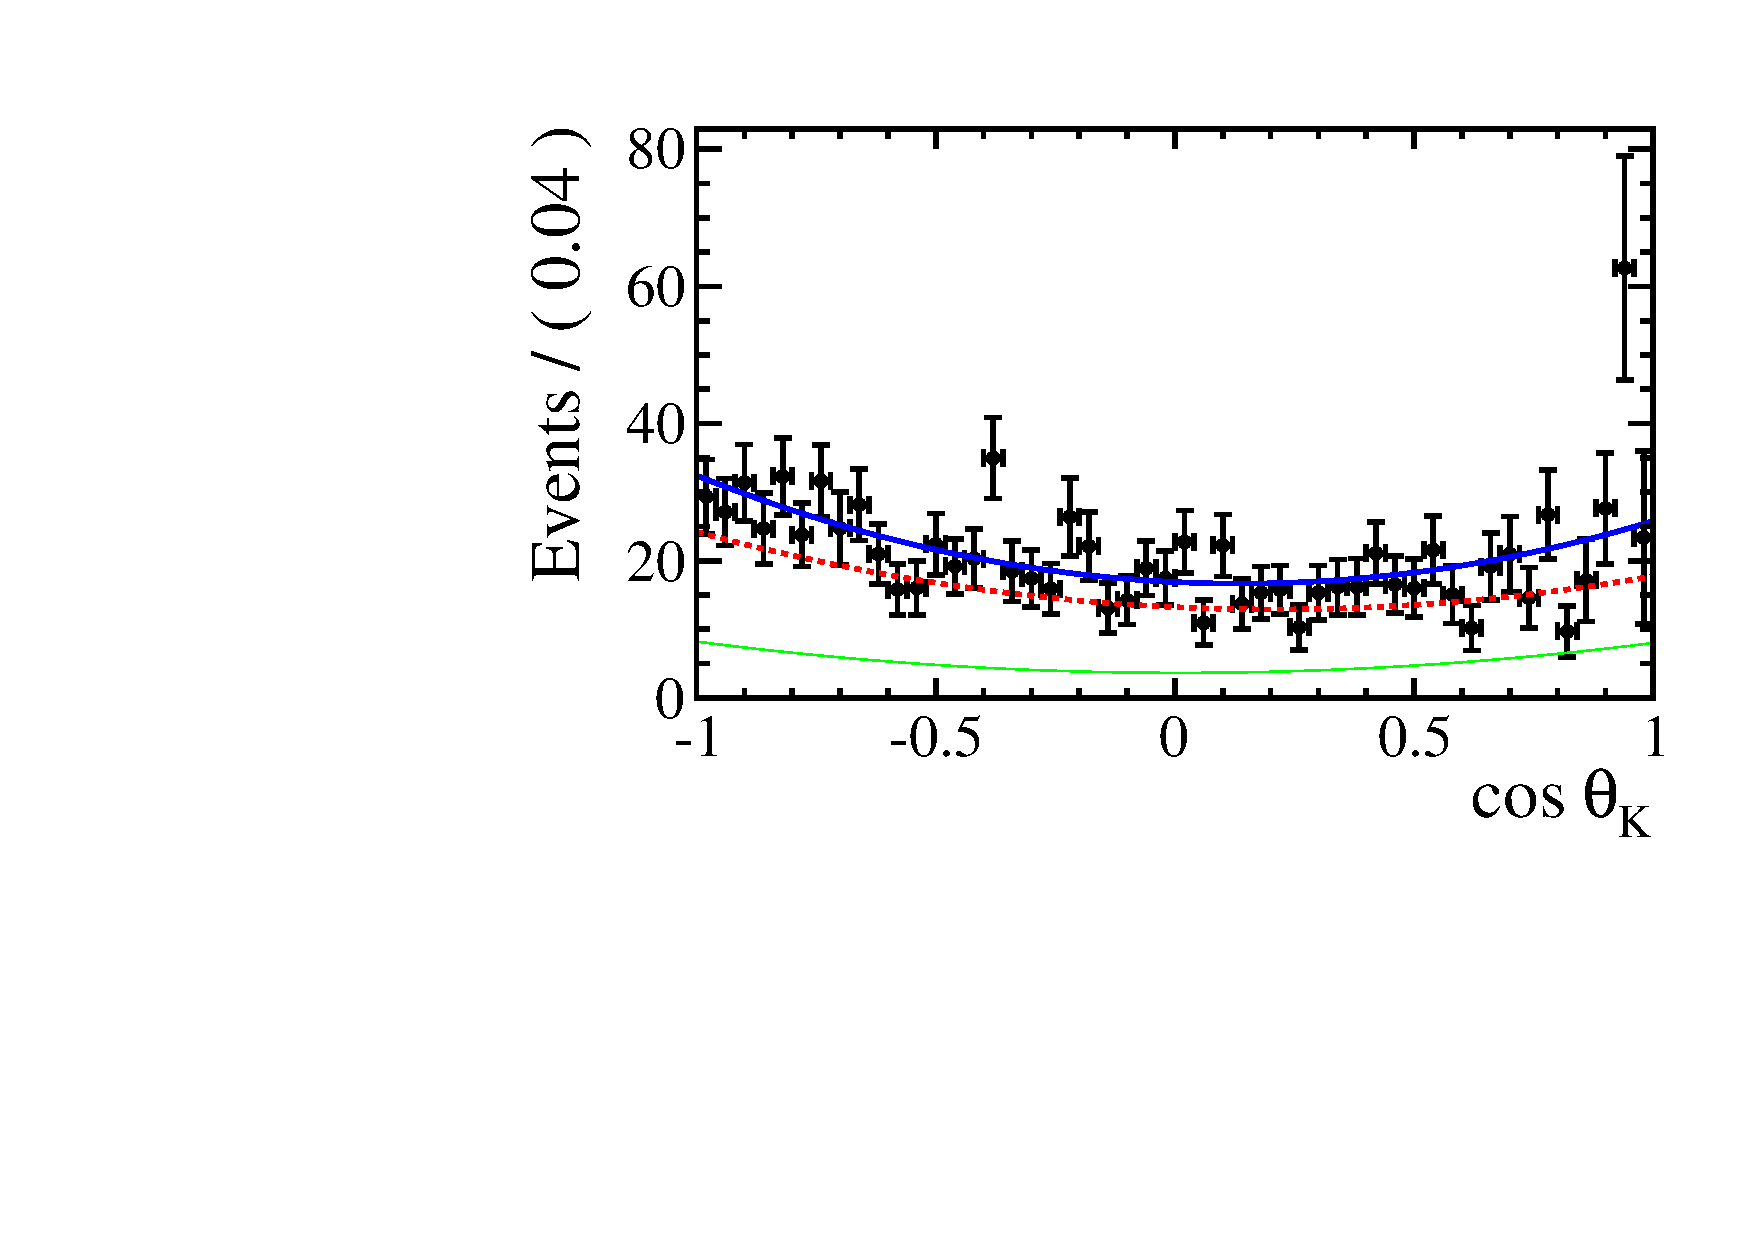
\includegraphics[width=0.48\columnwidth]
{chapter7/figs/fits/lass/fit_kstarmumu_swave_mkpi_range_lass_costhetak_canvas_6.pdf}}
\caption{ The result of the fit to the \qsq region from 1 to 6 \gevgevcccc. }
\end{figure}

\begin{figure}[tbp]
\centering
\subfigure{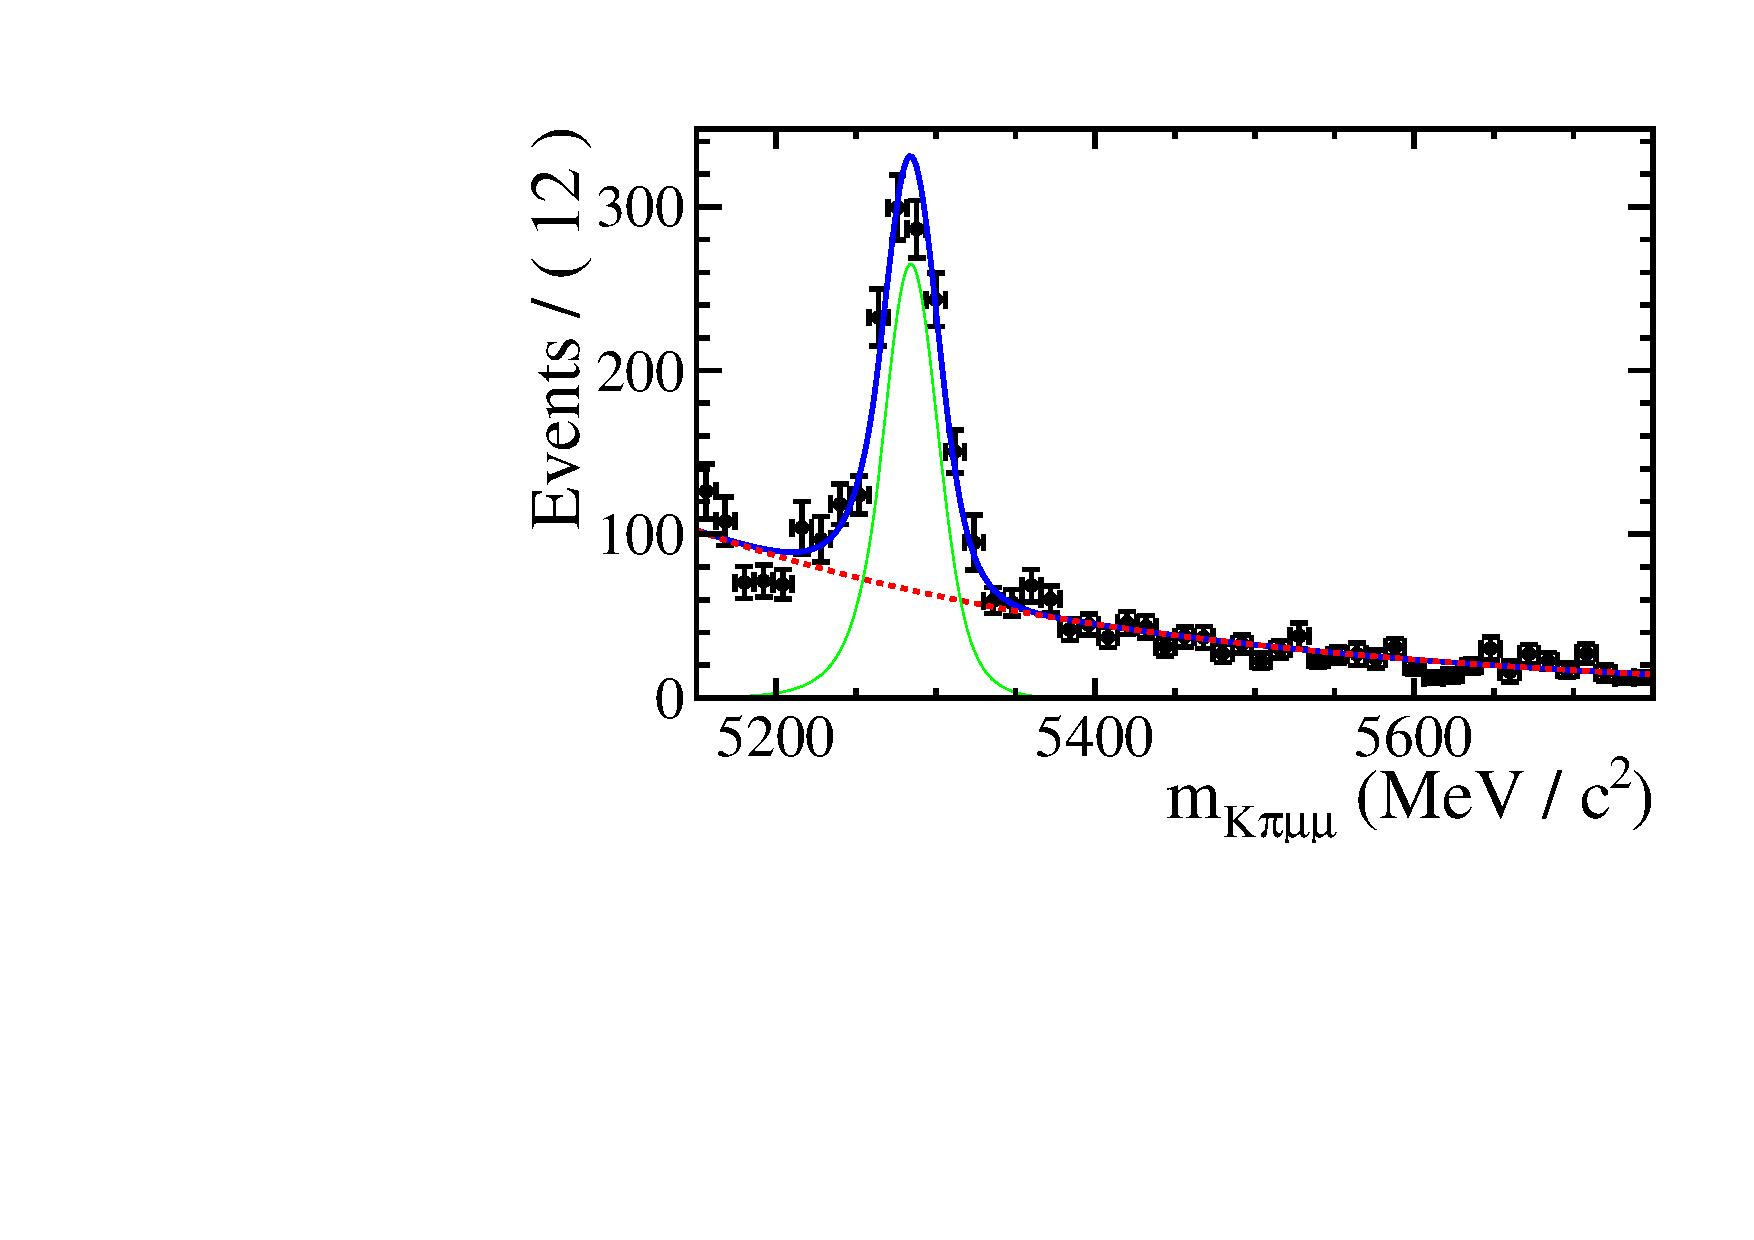
\includegraphics[width=0.48\columnwidth]
{chapter7/figs/fits/lass/fit_kstarmumu_swave_mkpi_range_lass_mass_canvas_7.pdf}}
\subfigure{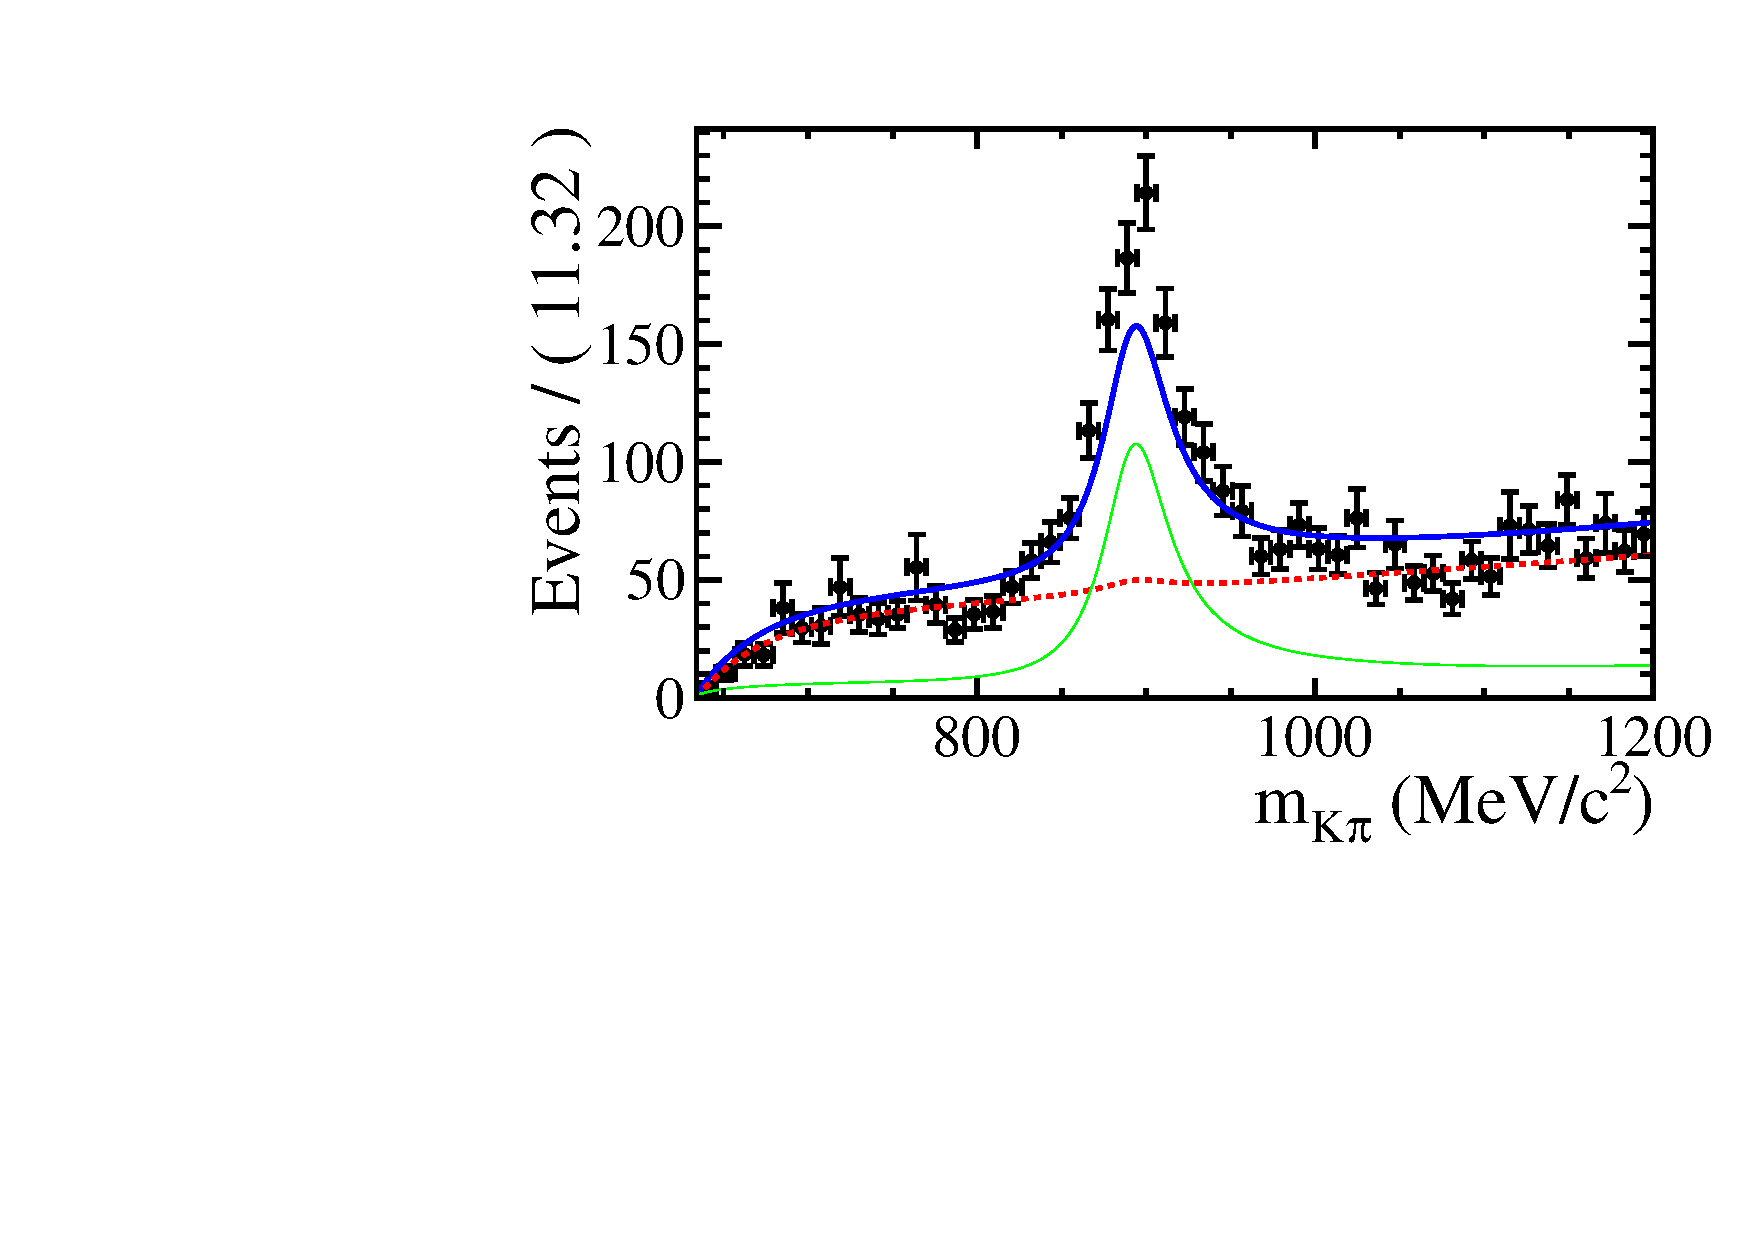
\includegraphics[width=0.48\columnwidth]
{chapter7/figs/fits/lass/fit_kstarmumu_swave_mkpi_range_lass_mkpi_canvas_7.pdf}}
\subfigure{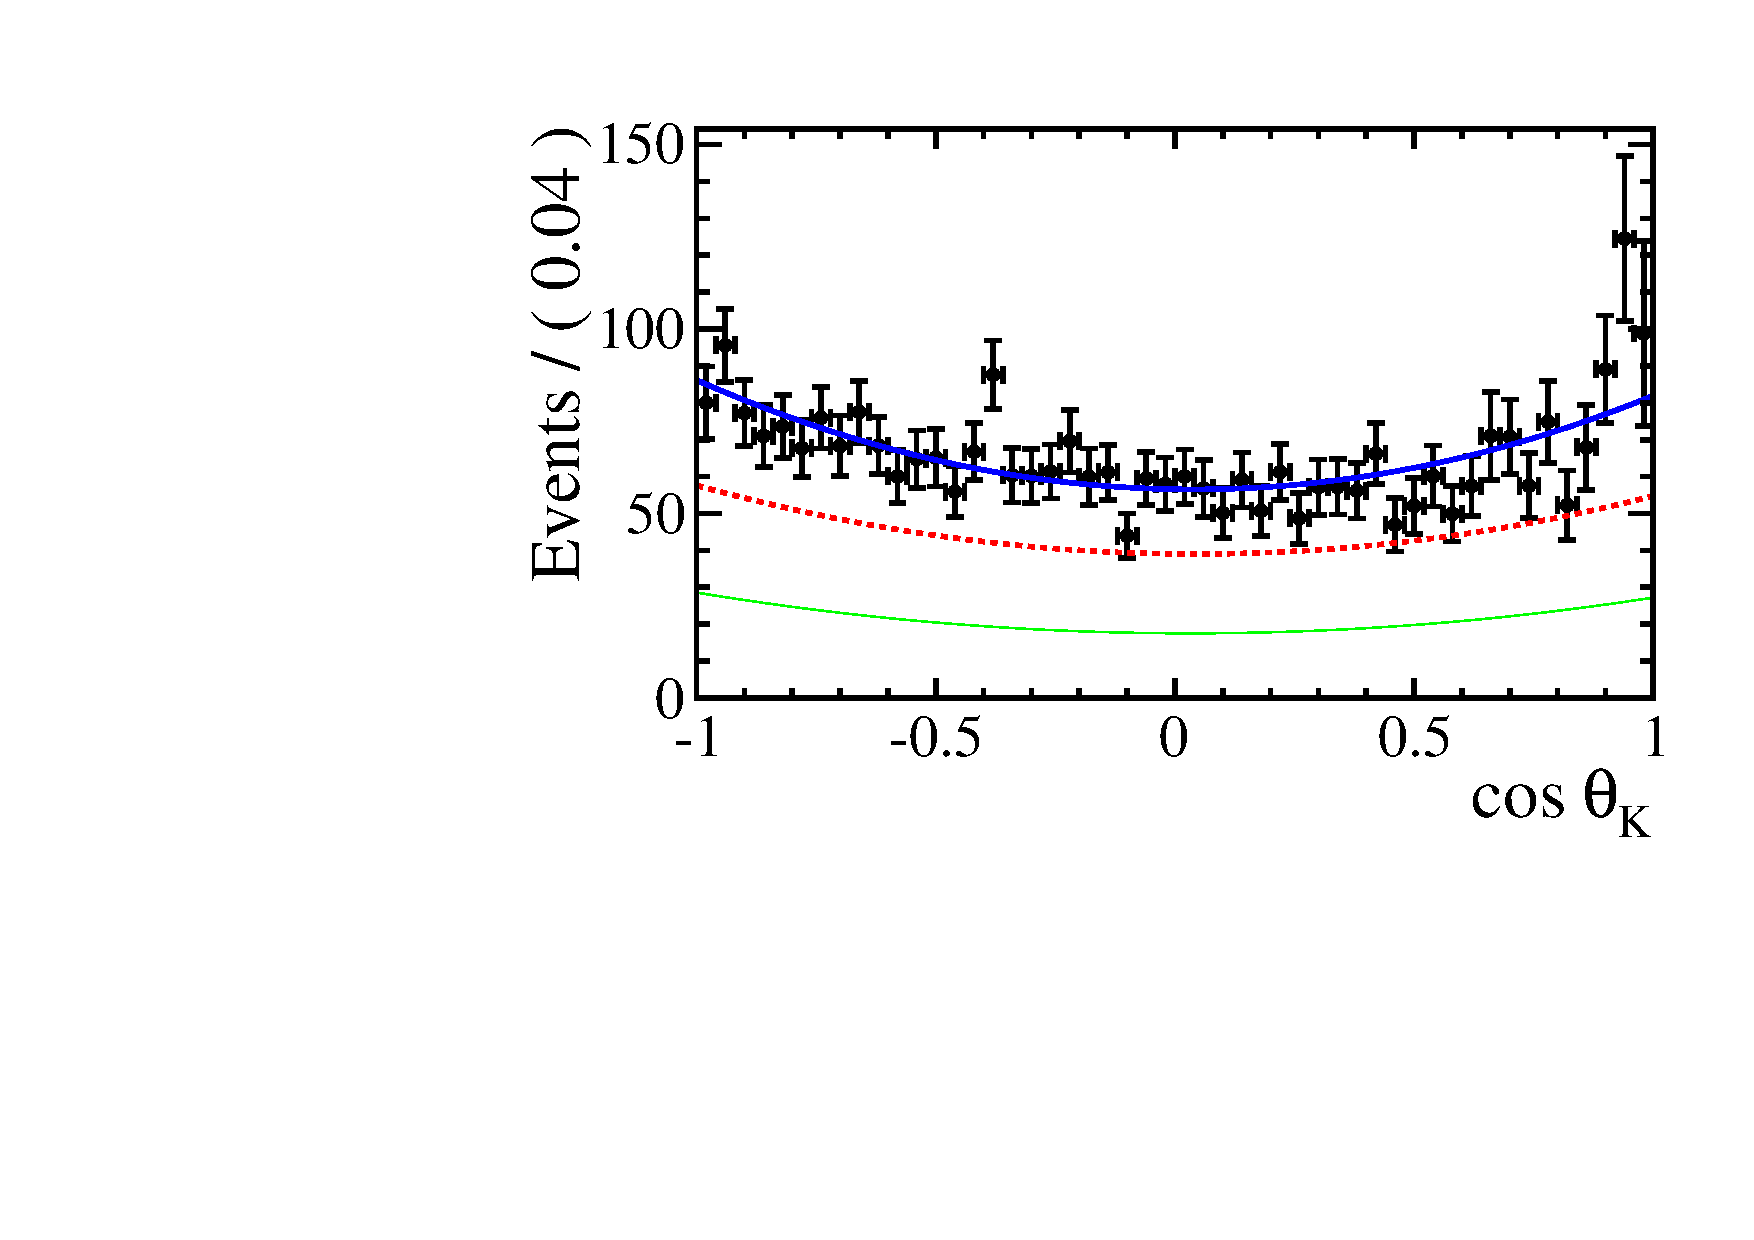
\includegraphics[width=0.48\columnwidth]
{chapter7/figs/fits/lass/fit_kstarmumu_swave_mkpi_range_lass_costhetak_canvas_7.pdf}}
\caption{ The result of the fit to the \qsq region from 0.1 to 19 \gevgevcccc. }
\end{figure}

\doublepage


\section{Isobar model}

\begin{figure}[tbp]
\centering
\subfigure{\includegraphics[width=0.48\columnwidth]
{chapter7/figs/fits/isobar/fit_kstarmumu_swave_mkpi_range_isobar_mass_canvas_0.pdf}}
\subfigure{\includegraphics[width=0.48\columnwidth]
{chapter7/figs/fits/isobar/fit_kstarmumu_swave_mkpi_range_isobar_mkpi_canvas_0.pdf}}
\subfigure{\includegraphics[width=0.48\columnwidth]
{chapter7/figs/fits/isobar/fit_kstarmumu_swave_mkpi_range_isobar_costhetak_canvas_0.pdf}}
\caption{ The result of the fit to the \qsq region from 0.1 to 2 \gevgevcccc. }
\end{figure}

\begin{figure}[tbp]
\centering
\subfigure{\includegraphics[width=0.48\columnwidth]
{chapter7/figs/fits/isobar/fit_kstarmumu_swave_mkpi_range_isobar_mass_canvas_1.pdf}}
\subfigure{\includegraphics[width=0.48\columnwidth]
{chapter7/figs/fits/isobar/fit_kstarmumu_swave_mkpi_range_isobar_mkpi_canvas_1.pdf}}
\subfigure{\includegraphics[width=0.48\columnwidth]
{chapter7/figs/fits/isobar/fit_kstarmumu_swave_mkpi_range_isobar_costhetak_canvas_1.pdf}}
\caption{ The result of the fit to the \qsq region from 2 to 4.3 \gevgevcccc. }
\end{figure}

\begin{figure}[tbp]
\centering
\subfigure{\includegraphics[width=0.48\columnwidth]
{chapter7/figs/fits/isobar/fit_kstarmumu_swave_mkpi_range_isobar_mass_canvas_2.pdf}}
\subfigure{\includegraphics[width=0.48\columnwidth]
{chapter7/figs/fits/isobar/fit_kstarmumu_swave_mkpi_range_isobar_mkpi_canvas_2.pdf}}
\subfigure{\includegraphics[width=0.48\columnwidth]
{chapter7/figs/fits/isobar/fit_kstarmumu_swave_mkpi_range_isobar_costhetak_canvas_2.pdf}}
\caption{ The result of the fit to the \qsq region from 4.3 to 8.68 \gevgevcccc. }
\end{figure}

\begin{figure}[tbp]
\centering
\subfigure{\includegraphics[width=0.48\columnwidth]
{chapter7/figs/fits/isobar/fit_kstarmumu_swave_mkpi_range_isobar_mass_canvas_3.pdf}}
\subfigure{\includegraphics[width=0.48\columnwidth]
{chapter7/figs/fits/isobar/fit_kstarmumu_swave_mkpi_range_isobar_mkpi_canvas_3.pdf}}
\subfigure{\includegraphics[width=0.48\columnwidth]
{chapter7/figs/fits/isobar/fit_kstarmumu_swave_mkpi_range_isobar_costhetak_canvas_4.pdf}}
\caption{ The result of the fit to the \qsq region from 10.06 to 12.9 \gevgevcccc. }
\end{figure}

\begin{figure}[tbp]
\centering
\subfigure{\includegraphics[width=0.48\columnwidth]
{chapter7/figs/fits/isobar/fit_kstarmumu_swave_mkpi_range_isobar_mass_canvas_4.pdf}}
\subfigure{\includegraphics[width=0.48\columnwidth]
{chapter7/figs/fits/isobar/fit_kstarmumu_swave_mkpi_range_isobar_mkpi_canvas_4.pdf}}
\subfigure{\includegraphics[width=0.48\columnwidth]
{chapter7/figs/fits/isobar/fit_kstarmumu_swave_mkpi_range_isobar_costhetak_canvas_4.pdf}}
\caption{ The result of the fit to the \qsq region from 14 to 16 \gevgevcccc. }
\end{figure}

\begin{figure}[tbp]
\centering
\subfigure{\includegraphics[width=0.48\columnwidth]
{chapter7/figs/fits/isobar/fit_kstarmumu_swave_mkpi_range_isobar_mass_canvas_5.pdf}}
\subfigure{\includegraphics[width=0.48\columnwidth]
{chapter7/figs/fits/isobar/fit_kstarmumu_swave_mkpi_range_isobar_mkpi_canvas_5.pdf}}
\subfigure{\includegraphics[width=0.48\columnwidth]
{chapter7/figs/fits/isobar/fit_kstarmumu_swave_mkpi_range_isobar_costhetak_canvas_5.pdf}}
\caption{ The result of the fit to the \qsq region from 16 to 19 \gevgevcccc. }
\end{figure}

\begin{figure}[tbp]
\centering
\subfigure{\includegraphics[width=0.48\columnwidth]
{chapter7/figs/fits/isobar/fit_kstarmumu_swave_mkpi_range_isobar_mass_canvas_6.pdf}}
\subfigure{\includegraphics[width=0.48\columnwidth]
{chapter7/figs/fits/isobar/fit_kstarmumu_swave_mkpi_range_isobar_mkpi_canvas_6.pdf}}
\subfigure{\includegraphics[width=0.48\columnwidth]
{chapter7/figs/fits/isobar/fit_kstarmumu_swave_mkpi_range_isobar_costhetak_canvas_6.pdf}}
\caption{ The result of the fit to the \qsq region from 1 to 6 \gevgevcccc. }
\end{figure}

\begin{figure}[tbp]
\centering
\subfigure{\includegraphics[width=0.48\columnwidth]
{chapter7/figs/fits/isobar/fit_kstarmumu_swave_mkpi_range_isobar_mass_canvas_7.pdf}}
\subfigure{\includegraphics[width=0.48\columnwidth]
{chapter7/figs/fits/isobar/fit_kstarmumu_swave_mkpi_range_isobar_mkpi_canvas_7.pdf}}
\subfigure{\includegraphics[width=0.48\columnwidth]
{chapter7/figs/fits/isobar/fit_kstarmumu_swave_mkpi_range_isobar_costhetak_canvas_7.pdf}}
\caption{ The result of the fit to the \qsq region from 0.1 to 19 \gevgevcccc. }
\end{figure}

